
%% Template Elsevier for Neuroimage

%% Use the option review to obtain double line spacing
%\documentclass[authoryear,preprint,review]{elsarticle}
\documentclass[authoryear]{elsarticle}
%\usepackage[framed,numbered,autolinebreaks,useliterate]{mcode}
\usepackage[framed,autolinebreaks,useliterate]{mcode}
\usepackage{natbib}
\usepackage{amsmath}
%\usepackage{lineno}
\usepackage{rotating}

\usepackage{hyperref}
\usepackage{amssymb}
\usepackage{amsfonts}


%\usepackage{algorithm2e}
%\usepackage{algorithmic}
%\usepackage{todonotes}
\usepackage{pdflscape}
\journal{Neuroimage}
\usepackage{color,transparent}
%\usepackage{color} 
%\pdfoptionpdfminorversion 6
\pdfminorversion=5

\usepackage{graphicx}
\usepackage{subcaption}
\usepackage{mwe}

\begin{document}

% Title must be 150 words or less
\begin{frontmatter}
\title{Feasibility of multi-centric fMRI connectivity studies of Alzheimer's disease}
%\title{A power analysis for multisite studies in resting-state functional connectivity, with an application to clinical trials in Alzheimer's disease}

\author[a,b]{Christian~Dansereau}
\author[c]{Celine~Risterucci}
\author[c]{Emilio~Merlo Pich}
\author[d]{Douglas~Arnold}
\author[a,b]{Pierre~Bellec\corref{cor1}}
\ead{pierre.bellec@criugm.qc.ca}
\cortext[cor1]{Corresponding author}
\address[a]{Centre de Recherche de l'Institut Universitaire de G\'eriatrie de Montr\'eal, Montr\'eal, CA}
\address[b]{D\'epartement d'Informatique et de recherche op\'erationnelle, Universit\'e de Montr\'eal, Montr\'eal,CA}
\address[c]{F. Hoffmann-La Roche Ldt., Basel, Switzerland}
\address[d]{NeuroRx, Montreal, Quebec, Canada}

% Please keep the abstract between 250 and 300 words
\begin{abstract}


\end{abstract}

%-- 
\begin{keyword}
fmri \sep general linear model \sep effect size \sep multiple comparison \sep multisite \sep clinical trial analysis
\end{keyword}
\end{frontmatter}

% Unique number for each line
%\linenumbers
%\listoftodos

\section*{Highlights}

\begin{itemize}
\item etc
 %\item The impact of the number of nodes, or scale, on the sensitivity of a connectome-wide association study is systematically evaluated.
 %\item A procedure is presented that controls the false-discovery rate within- and between scales.
 %\item The technique is evaluated on a simulation of multiscale changes in connectome organization.
 %\item The technique is applied on three different datasets, for which there is a good a priori knowledge on the underlying connectivity changes.
 %\item Several recent procedures for connectome-wide association are compared.
\end{itemize}

\section{Introduction}

% Magic paragraph
Resting-state (RS) connectivity in fMRI is a promising biomarker for a variety of neurological diseases. Typically, in a clinical trial, a large cohort is recruited and evaluated at multiple sites spread over countries or even continents. The main potential issue with that approach is the lack of consistency in the multi-site RS connectivity acquisitions that may obscure clinically relevant information. Therefore the aims of the study were to: (1) characterize the amplitude of the site bias, i.e. the systematic differences in rs-fMRI connectivity across different acquisition sites; (2) Quantify the impact of the between-site variance on the power of statistical tests in resting-state fMRI.

The number of Canadians suffering from Alzheimer's disease (AD) is rapidly increasing, with tremendous social and economic impact. Despite the emergence of promising drugs, the recent clinical trials with demented patients have failed. Dementia however comes very late in the development of the disease, at a stage where the degeneration of neural tissues has likely gone beyond repair. In order to be efficient, therapies should be initiated in the decades predating dementia, in a preclinical stage where patients experience no or very mild symptoms (see chapter $1.1$). There are unfortunately no biomarker(s) that are currently predictive of AD in this preclinical stage, and could help identify the individuals that could benefit from such interventions. A promising technique is resting-state functional magnetic resonance imaging (rs-fMRI), which may be able to capture the early synaptic dysfunction seen in AD (see chapter $1.2$). I order to be able to apply statistical analysis and machine learning methods we 
need to preprocess the data to remove as much as possible the effect of various artefacts (hardware and physiological). The preprocessing reduces the variability of the data and therefore provides more relevant and discriminative features (see chapter $1.3$). In order to further improve the statistical power of there analysis, multiple academic groups are collaborating to pool their dataset to increase the sample size of the study. Unfortunately the gain in sample size comes with a new source of variability introduced by the multicentric acquisition. Site-specific MRI set-ups may bias the fMRI measures, and I am thus developing procedures for inter-site normalization. Account for these sources of variance are important since they may bias the predictive potential of rs-functional connectivity in a multi-site, in line with this last assumption we want to quantify the robustness of the feature selection and classifier to multi-site acquisition (see chapter $1.4$).

In most experiments conducted in neuroimaging, the main factors that influence power are: (1) the size of the effect, determined by the difference of the mean connectivity of one group versus a control group and the variability of this difference across subjects and groups; and (2) the sample size, i.e. the number of subjects in the study \citep{Desmond2002}. This last factor is usually the only one controlled by the investigator, hence why an increasing number of researchers share multicentric, sometimes multiprotocol, data suitable to statistical analysis. In research it is very difficult to obtain a grant large enough to scan a cohort larger than ~80 subjects, therefore researcher and consortium initiatives have started to pool their resources together to make initiative composed of publicly available large cohorts of subjects like the 1000 functional connectome \citep{Biswal2010}, ADNI \citep{
Mueller2005}, among 
others. In clinical trial the justification for multicentric acquisition is more of a logistical one then a financial reason; they need to recruit a large amount of subject in a short period of time. In order to achieve this goal they mandate the recruitment to multiple clinical centers across the globe which accelerate the evaluation time of a drug. Although these centers may be similar by their scanner protocols, scanners will have difference in their software version, specific add-on to the scanners, and, most importantly, vendors (even field strength may differ in some cases). Unfortunately between studies, MR acquisition methodologies are among the most commonly cited sources of measurement variation \citep{Friedman2006}. This is why it is important to assess if multi-site resting-state connectivity analysis are feasible (we can combine the data from multiple sources while introducing a reasonable amount of variance which is still acceptable to detect effects in the data) and what corrective measure on 
the data should be applied to reduce the bias introduced by multi-site analysis. Among the factor of variability across sites, we can list the following 3 categories described in \citep{Yan2013a}:


\textit{
\begin{enumerate}
\item Acquisition-related variations:
\begin{enumerate}
\item Scanner make and model \citep{Friedman2006}
\item Sequence type (spiral vs. echo planar; single-echo vs. multi-echo) \citep{Klarhoefer2002}, parallel vs. conventional acquisition \citep{Feinberg2010} \citep{Lin2005}
\item Coil type (surface vs. volume, number of channels, orientation).
\item Acquisition parameters: repetition time, number of repetitions, flip angle, echo time, and acquisition volume (field of view, voxel size, slice thickness/gaps, slice prescription) \citep{Friedman2006a}.
\end{enumerate}
\item Experimental-related variations: 
\begin{enumerate}
\item Participant instructions \citep{Hartstra2011}, eyes-open/eyes-closed \citep{Yan2009} \citep{Yang2007}, visual displays, experiment duration \citep{Fang2007} \citep{VanDijk2010}.
\end{enumerate}
\item Environment-related variations: 
\begin{enumerate}
\item Sound attenuation measures \citep{Cho1998} \citep{Elliott1999}.
\item Attempts to improve participant comfort during scans (e.g., music, videos) \citep{Cullen2009}.
\item Head-motion restraint techniques (e.g., vacuum pad, foam pad, bite-bar, plaster cast head holder) \citep{Edward2000} \citep{Menon1997}.
\item Room temperature and moisture \citep{Vanhoutte2006}.
\end{enumerate}
\end{enumerate}
}

In 2009, the publicly released 1000 Functional Connectomes Project (FCP) and International Neuroimaging Data-sharing Initiative (INDI) provided a glimpse of the variability in imaging methodologies employed by the neuroimaging field. The dataset includes rs-fMRI samples independently collected at imaging sites around the world. A noteworthy aspect of this dataset is the variation in almost every parameter of the imaging acquisition methodologies, while the majority of subject-related variables are not reported (due in most cases, to the fact that they were not thoroughly recorded). 
Despite justifiable scepticism, feasibility analyses demonstrated that meaningful explorations of the aggregate dataset, composed of 24 imaging sites for a grand total of 1093 subjects, could be performed \citep{Biswal2010}. Although no explicit correction for multi-site variability was used, they only use global signal correction (GSC) to normalize subjects which may introduce anti-correlation in the data \citep{Fox2009, Murphy2009, Saad2012, Carbonell2014, Power2014}. After accounting for site-related differences, the analysis showed brain-behaviour relationships with phenotypic variables such as age, gender, and diagnostic label, and confirmed a variety of prior hypotheses \citep{Biswal2010, Fair2012, Tomasi2010, Zuo2012}. While encouraging, many uncontrolled and unknown factors in the 1000 FCP remain a source of concern, as they spread beyond simple site effects and can limit the datasets utility as highlighted by \cite{Yan2013}.
An other compelling proof of multi-site bias is the study reported by \cite{Nielsen2013} where they did an analysis on a single site dataset and a multi-site dataset of subject with autism and concluded that the multi-site autism study classification accuracy significantly outperformed chance but was much lower for multi-site prediction than for previous single site results \citep{Nielsen2013}. We therefore need to keep in mind that the site effect must be taken in account in the analysis or we may reduce our detection power.

\paragraph{Specific objectives} 

\begin{itemize}
 \item Propose methods to account for multisite variance in a general linear model analysis
 \item Amount of variance intra-site and inter-site
 \item How group balancing in multi-centric topology impact sensitivity
 \item How sample size in multi-centric topology impact sensitivity
 \item Interaction of 
\end{itemize}


\section{Method}

\subsection{Data samples} 
\paragraph{Participants}
The paper studies 313 elderly adults with and without cognitive impairment of the Alzheimer type collected across 5 studies: ADNI2 study and 4 other studies based in Montreal, Canada (from the ADMTL dataset), for a grand total of 126 CNE participants (51 males, age range = 57-94 yrs), 133 patients with MCI (70 males, age range = 55-89 yrs), and 54 patients with DAT (22 males, age range = 55-88 yrs) (see table \ref{tab_retention}).
We have also included 355 cognitively normal young adults (CNY) from the 1000 functional connectome project\footnote{\url{http://fcon_1000.projects.nitrc.org/}} (150 males, age range = 18-46 yrs) as a reference dataset.

\paragraph{Acquisition} %Resting-state scans were acquired on a 3T Siemens TrioTim for all datasets. One single run was obtained per subject for either the SCHIZO or BLIND dataset while two runs were acquired in each subject for the MOTOR dataset, one immediately preceding and one following the practice on a motor task. 
%For the 1000 functional connectom dataset, 150 EPI volumes were recorded in 6 mins 40 s (TR = 2.65s, TE = 30ms, FA = 90\textdegree, 43 slices, voxel size = 3.4x3.4x3 mm$^3$, gap = 10\%, matrix size = 64x64, FOV = 220x220 mm$^2$), and a structural image was acquired using a MPRAGE sequence (TR = 2.3~s, TE = 2.98~ms, FA = 9\textdegree, 176 slices, voxel size = 1x1x1 mm$^3$, matrix size = 256x256, FOV = 256x256 mm$^2$).

\subsection{Preprocessing}\label{Preprocessing}
The datasets were analysed using the NeuroImaging Analysis Kit (NIAK\footnote{\url{http://www.nitrc.org/projects/niak/}}) version 0.12.14, under CentOS version 6.3 with Octave\footnote{\url{http://gnu.octave.org}} version 3.8.1 and the Minc toolkit\footnote{\url{http://www.bic.mni.mcgill.ca/ServicesSoftware/ServicesSoftwareMincToolKit}} version 0.3.18. Analyses were executed in parallel on the "Mammouth" supercomputer\footnote{\url{http://www.calculquebec.ca/index.php/en/resources/compute-servers/mammouth-parallele-ii}}, using the pipeline system for Octave and Matlab \citep{Bellec2010}, version 1.0.2. Brain map visualizations were created using MRICron software \cite{Rorden2007}. Each fMRI dataset was corrected of inter-slice difference in acquisition time and the parameters of a rigid-body motion was estimated for each time frame. Rigid-body motion was estimated within as well as between runs, using the median volume of the first run as a target. The median volume of one selected fMRI run for each subject 
was 
coregistered with a T1 individual scan using Minctracc \citep{Collins1998}, which was itself non-linearly transformed to the Montreal Neurological Institute (MNI) template \citep{Fonov2011} using the CIVET pipeline \citep{Zijdenbos2002}. The MNI symmetric template was generated from the ICBM152 sample of 152 young adults, after 40 iterations of non-linear coregistration. The rigid-body transform, fMRI-to-T1 transform and T1-to-stereotaxic transform were all combined, and the functional volumes were resampled in the MNI space at a 3 mm isotropic resolution. The a censoring method described in \citep{Power2012} called "scrubbing" was used to remove the volumes with excessive motion using a cut-off value of $FD\geq0.5$. A minimum number of 50 unscrubbed volumes per run, corresponding to $\sim 125$ s of acquisition for a TR of 2.5 seconds, was then required for further analysis. The following nuisance parameters were regressed out from the time series at each voxel: slow time drifts (basis of discrete cosines 
with a 0.01 Hz high-pass cut-off), average signals in conservative masks of the white matter and the lateral ventricles as well as the first principal components (95\% energy) of the six rigid-body motion parameters and their squares \citep{Lund2006},\citep{Giove2009}. The fMRI volumes were finally spatially smoothed with a 6 mm isotropic Gaussian blurring kernel. 

\subsection{Feature selection}
Regions are routinely defined using an anatomical parcellation \citep{He2009}, such as the AAL template \citep{Tzourio-Mazoyer2002}. Anatomical parcels may however not well match the organization of resting-state networks. The BASC method was used to generate data-driven functional decomposition into resting-state networks based on the coherence of BOLD activity at the individual or group level \citep{Bellec2006,Bellec2010c,Bellec2013}. When a low number of networks (or scale) is used, the brain got decomposed into distributed large-scale networks, such as the DMN. At high scales (large number of networks), the BASC identified subnetworks and functional regions \citep{Kelly2012}. We generated a BASC parcellation in 100 clusters on the Cambridge sample, including $\sim 200$ young adults from the 1000 functional connectome database \citep{Biswal2010} and used it to generate the rs-fMRI outcome measures.

\paragraph{The default-mode network}
Since the seminal work of \cite{Greicius2004}, many rs-fMRI studies in AD focused on the default-mode network (DMN), a group of regions consistently more active at rest than during a broad range of different tasks \citep{Gusnard2001}. The DMN was notably reported to largely overlap with the regions that show high amyloid-beta deposition in patients with DAT \citep{Buckner2009}. It includes the posterior cingulate cortex (PCC) / Precuneus (PCUN) area, the inferior parietal lobule (IPL), the anterior cingulate cortex / medial prefrontal cortex (MPFC) \citep{Greicius2003}. Other structures such as the medial temporal cortex or the superior frontal gyrus are also generally regarded as part of different subnetworks of the DMN \citep{Margulies2009, Andrews-Hanna2010a}.

\paragraph{Literature review: Alzheimer's disease and resting-state fMRI}
We performed a literature review to select candidate connections that have been shown to be prominently impacted in Alzheimer's disease. There is no single authoritative reference on the effect of a DAT on rs-fMRI connectivity, and the field has been dominated thus far by studies with small samples (n\textasciitilde20) and limited statistical power, see \cite{Sheline2013} for a recent review. Because the DMN has been most extensively studied, we decided to focus on this network and to run a meta-analysis on six papers that (1) used some analogue of seed-based connectivity maps in resting-state fMRI using one or multiple seeds in the DMN (2) investigated abnormalities in resting-state functional connectivity in patients suffering of a dementia of the Alzheimer's type and (3) provided tables of coordinates in stereotaxic space for the results.

\paragraph{review: Alzheimer's disease and resting-state fMRI} 
\begin{itemize}
\item \cite{Zhang2009a} used functional connectivity maps with a seed in the posterior cingulate cortex (PCC) to explore the differences between a group of elderly cognitively normal subjects (CNE, n=16) and patients with a mild dementia of the Alzheimer's type (DAT, n=18).
\item \cite{Zhang2010} generalized the \cite{Zhang2009a} study with CNE (n=16) and a larger group of patients with DAT (n=46). Patients were separated in three groups (mild, moderate, severe DAT), and each group of patients was contrasted against the CNE.
\item \cite{Wang2006a} used functional connectivity maps with a seed in the hippocampi to explore the differences between a group of CNE (n=13) and patients with a mild DAT (n=13). All results included in the meta-analysis are from Table 2, seeded in the right hippocampus. Seeds were manually delineated on an individual basis.
\item \cite{Wang2007a} used functional connectivity maps with a seed in the posterior cingulate cortex (PCC) as well as full brain point-to-point correlations (based on an AAL parcellation) to explore the differences between a group of elderly cognitively normal subjects (CNE, n=14) and patients with a very mild to mild dementia of the Alzheimer's type (DAT, n=14). Only the results based on the PCC seed were included in the meta-analysis.
\item \cite{Goveas2011} used functional connectivity maps with a seed in the hippocampi to explore the differences between a group of elderly cognitively normal subjects (CNE, n=18) and patients with a mild dementia of the Alzheimer's type (DAT, n=14) before and after donepezil treatment. Seeds were manually delineated on an individual basis, before and after treatment.
\item \cite{Damoiseaux2012} used dual-regression independent component analysis to explore longitudinal differences between a group of CNE (n=18) and patients with DAT (n=21). All results included in the meta-analysis are from Table 3 (differences at baseline) and Table 4 (interaction with time). The authors used three components representing the Anterior DMN, Ventral DMN and Posterior DMN.
\end{itemize}

To assess the degree of consistency of the findings across studies, we counted the number of coordinates located in each one of the BASC regions. The resulting map is presented in Figure \ref{fig_freq_sel}. As can be seen, there is a lot of variability across studies, with only a limited number of regions reaching a score above 3 (i.e. reported in at least 3 of the contrasts in the six studies). Note that we did not select connections with the hippocampus, although this region was frequently reported. The rationale was that the drug effects on this area are expected to be minimal in patients with a moderate DAT, because the very severe atrophy of the structure cannot be recovered. In the regions showing the most consistency (score of 3 or more), there were many regions located in the DMN, such as the PCC, the PCUN, the IPL (a bilateral node), the right superior frontal gyrus (SFGr), as well as two dorsal MPFC cortex (dMPFC and dMPFC2) and an anterior MPFC parcel (aMPFC). Three parcels were found in the 
visual network: the lingual gyrus (LING), the fusiform gyrus (FUS) and a dorso-medial occipital (DMO) parcel. Two parcels were found in the dorsal attentional network: the intra-parietal sulcus (IPS) and the motor part of the precuneus (PCUNm, see \cite{Margulies2009}). One parcel was found in the premotor cortex (PMC), associated with the sensorimotor network, one parcel in the left dorsolateral prefrontal cortex (rDLPFC), associated with the fronto-parietal task-control network, as well as a parcel in the dMPFC (dMPFC3) associated with the cingulo-opercular cortex. Finally, a parcel included the temporal poles (TPo) bilaterally. Note that the nomenclature for distributed networks was based on \citep{Power2011}. 

The TRT reliability study was based on the publicly available NYU-TRT database. The database included 25 young healthy adults, and each subject had three rs-fMRI run: two in a single session (separated by 45 mns) and another run $5-16$ months latter. Several outcome measures were generated in key regions impacted by AD. Using the three runs, one intra-class correlation (ICC) was generated intra-session, and two ICCs were generated inter-session for each outcome measures. The outcome measures were ranked based on average of intra- and inter-session ICCs. 

\subsection{Simulations}


\paragraph{Parcellation}
Functional brain parcellation into 300 regions was obtained from reference dataset of healthy adults from the 1000 functional connectome project (Cambridge cohort, parcelation available here \ref{}). To do so the spatial dimension of the independent individual fMRI dataset was reduced to 957 regions using a region-growing algorithm \cite{Bellec2006} and final network decomposition was obtained using BASC \cite{Bellec2010c} a bootstrap method to identify stable networks at various scales.

\subsection{Functional network}
Regions are routinely defined using an anatomical parcellation \citep{He2009}, such as the AAL template \citep{Tzourio-Mazoyer2002}. Anatomical parcels may however not well match the organization of resting-state networks. We use a framework to generate data-driven functional decomposition into resting-state networks based on the coherence of BOLD activity at the individual or group level \citep{Bellec2006},\citep{Bellec2010c}. When a low number of networks (or scale) is used, this technique, called bootstrap analysis of stable clusters (BASC), generates decompositions of the brain into distributed large-scale networks, such as the DMN. At high scales, it identifies subnetworks and functional regions \citep{Kelly2012}. We generated a BASC parcellation with a 100 clusters on the Cambridge sample, including $\sim$ 200 young adults from the 1000 functional connectome database \citep{Biswal2010} and used it to generate the rs-fMRI outcome measures.

\paragraph{Functional maps}
For each run, the correlation matrix was generated base on the time series averaged on the parcellation of an independent dataset mention previously (Cambridge 100 parcels). For each subject, the connectomes were averaged across all runs. The following region posterior cingulate cortex (PCC), a central node of the default mode network, was used to generate seed based connectivity maps. Finally, the average voxelwise functional connectivity maps was generated, i.e. Pearson's correlation corrected by the Fisher transform and averaged across all runs for each subject.


\subsection{Statistical analysis}  

\paragraph{Dataset}
In order to simulate various scenarios within the context of a multi-site setting, a cohort of subjects acquired at a single-site was selected to act as our reference dataset and for the multi-site configuration a cohort from a collection of 7 small sites, roughly totalling the same sample size as the reference dataset, was used. The cohort used for the study contains 385 participants from the 1000 Functional Connectomes Project \citep{Biswal2010} (150 males, age range = 18-46 yrs) composed of 1 large site (Cambridge n=\textasciitilde200) and 7 small sites (n=\textasciitilde20/site for a total \textasciitilde200). The fMRI datasets were preprocessed with the Neuro-Imaging Analysis Kit (NIAK) as described earlier in Section \ref{Preprocessing}.

\paragraph{Functional connectome}
Using a brain partition of $R$ networks obtain from BASC procedure described in \cite{Bellec2010c}, and taking each pair of distinct networks $i$ and $j$, the between-network connectivity $y_{i,j}$ is measured by the Fisher transform of the Pearson's correlation between the average time series of the network. The within-network connectivity $y_{i,i}$ is the Fisher transform of the average correlation between time series of every pair of distinct voxels inside network $i$. The connectome $\mathbf{Y}=(y_{i,j})_{i,j=1}^R$ is thus a $R\times R$ matrix. Each column $j$ (or row, as the matrix is symmetric) codes for the connectivity between network $j$ and all other brain networks (full brain functional connectivity map). For a scale with $R$ parcels, there are exactly $L=R(R+1)/2$ distinct elements in an individual connectome $\mathbf{Y}$. 

\paragraph{Point-to-point connections}
Based on the literature review previously described the connectivity between 10 reproducible pair of regions were selected based on the criteria that they were impacted by the disease (specifically the pDAT-CNE contrast) in a literature review.

\paragraph{Estimation of the detection sensitivity}
The following confounding variables were modelled in the GLM analysis: frame displacement (FD), age and gender. Significance of the results is obtain with a Student $t$-test and the sensitivity of the test is evaluated by sub-sampling 70\% of the dataset ($B=10^4$ random samples). For each sample $b$, we have a $p$-value $p^{*}_b$ and the detection sensitivity is estimated by the probability of $p^{*}_b$ being inferior to $0.05$.
\begin{equation}\label{Detection power}  
    \frac{1}{B}\sum\limits_{b=1}^B\left(p^{*}_b\leq0.05\right).
\end{equation}


\paragraph{Effect size (cohen's d)}
For each site and each sample, half of the subjects were randomly assigned to a "treatment" group and a Monte-Carlo simulation was used to estimate the detection power in the single-site and in multi-site setting.

The normalized Cohen's d was used to estimate the effect size and it is defined as the difference between two means $\bar{x_{1}},\bar{x_{2}}$ divided by a standard deviation from the data $s$.

For each site an effect is added to the connectivity of 50\% of the subjects, selected randomly ("pathological" group):
\begin{equation}
	y_{i,j} = y_{i,j} + \mu.
\end{equation}

The parameter $\mu$ is chosen to obtain a particular effect size (measured by the Cohen $d$)
%The normalized Cohen's d was used to estimate the effect size and it is defined as the difference between two means $\bar{x_{1}},\bar{x_{2}}$ divided by a standard deviation from the data $s$.
%Le paramètre $\mu$ est choisi pour réaliser une certaine taille d'effet (mesuré par le $d$ de Cohen): %(difference entre deux moyenne $\bar{x_{1}},\bar{x_{2}}$) divisé par la deviation standard $s$.
\begin{equation}\label{cohen's d}
    \begin{array}{l l}
      d = \frac{\mu}{s_{i,j}},      
    \end{array}
\end{equation}
where $s_{i,j}$ is the standard deviation between region $i$ and $j$ for the reference population (mono-site, Cambridge). The significance of the difference between the control and 'treatment' group was assessed by a $t$-test in a linear model, including a covariate to model the motion. The study was repeated for various effect sizes (0 to 0.8 with a step of 0.01) with a $p$-value threshold of $0.05$ on the $t$-test.

%In order to introduce the same effect-size across the single-site and multi-site dataset we are taking the standard deviation from the single-site cohort as the reference.  The connection $y_{i,j}$ of the randomly affected subjects ("treatment" group) are therefore calculated $y_{i,j} = y_{i,j} + d\times s_{i,j}$. 

\paragraph{multi-site correction approaches} 

For the multi-site three flavours were computed: multi-site no correction, multi-site with dummy variables and multi-site with METAL correction.
Depending on the multi-site configuration and distribution of the subject we proposed two corrective approaches that can be applied as shown in the simulations of Figure \ref{fig_simu_50pct}. The first one is the introduction of dummy variables (binary vectors $1\times N$) who code for each site in the GLM model \ref{dummy variable equation}.

The variables are corrected to have a zero mean across subjects, and an intercept (i.e. a column filled with 1) is added to $\mathbf{X}$. The GLM relies on the following stochastic model:

 \begin{equation}
 \label{eq_glm}
  \mathbf{Y} = \mathbf{X}\mathbf{\beta} + \mathbf{V}\mathbf{\gamma}+ \mathbf{E},
 \end{equation}
 \begin{itemize}
  \item $\mathbf{Y}$: $N\times 1$, connectivity value for the pair ($i,j$),
  \item $\mathbf{X}$: $N\times K$, explainable variables,
  \item $\mathbf{\beta}$: $1 \times K$, regression values for each explainable variable,
  \item $\mathbf{V}$: $N\times S$, each column code for a site (0/1),
  \item $\mathbf{\gamma}$: $1\times S$, site average connectivity,
  \item $\mathbf{E}$: $N\times 1$, residual values from the regression,
 \end{itemize}
with $N$ the number of subjects, $K$ the number of explainable variables, $S$ the number of sites.

where $\mathbf{\beta}$ is an unknown $C\times L$ matrix of linear regression coefficients and $\mathbf{E}$ is a $N\times L$ random (noise) multivariate Gaussian variable. %As data generated from different subjects are statistically independent, and under an homoscedasticity assumption, the regression coefficients $\mathbf{B}$ can be estimated with ordinary least squares.
To apply the correction $v-1$ dummy-variables are added to the model \ref{dummy variable equation} with $v$ being the total number of sites used in the study.

The second approach is to compute the GLM independently on each site and then combine the statistical results from each site in a global score. This model averaging technique called METAL from \cite{Willer2010} model site specific bias by running a GLM analysis on each site resulting in $v$ beta vectors that are weighted proportionally to the standard error of each site and finally averaged as shown in equation \ref{METAL}. This is the most flexible way to account for multi-site effect wile keeping the analysis simple and robust to unbalanced sites.

\begin{equation}
	\beta_{v} \text{, effect size estimate for site \textit{v}.}
\end{equation}
\begin{equation}
	\sigma_{v} \text{, standard error for site} \textit{v}.
\end{equation}
\begin{equation}
 	w_{v}=\frac{1}{\sigma_{v}^{2}} \text{, weight estimate for site \textit{v}.}
 \end{equation}
 \begin{equation}
 	\beta=\frac{\Sigma_{v}\beta_{v}w_{v}}{\Sigma_{v}w_{v}} \text{, global }\beta.
 \end{equation}
  \begin{equation}
 	\sigma=\sqrt{\frac{1}{\Sigma_{v}w_{v}}} \text{, global standard error.}
 \end{equation}
\begin{equation}\label{METAL}
	Z=\frac{\beta}{\sigma} \text{, global Z score.}
\end{equation}
\begin{equation}
	p=2(1-\phi(\vert Z \vert) \text{, p-value.}
\end{equation}



\paragraph{Framewise displacement (FD)}
Index measure of head motion from one frame to the other. It is calculated as the sum of the absolute values of the differentiated realignment estimates at every time point \citep{Power2012} this measure give us an approximation of the motion frame by frame in millimeter. We are using this measure as an index of motion estimation.

\begin{equation}
    FD_{i} = \vert \triangle d_{x}(t) \vert + \vert \triangle d_{y}(t) \vert + \vert \triangle d_{z}(t) \vert + \vert \triangle r_x(t) \vert + \vert \triangle r_y(t) \vert + \vert \triangle r_z(t) \vert,
\end{equation}
\begin{equation}
  r_x(t) = 50\left(\frac{2\pi\alpha_x(t)}{360}\right),
\end{equation}
with 
\begin{itemize}
 \item ($d_x(t),d_{y}(t),d_{z}(t)$) translation parameters (mm),
 \item ($\alpha_x(t),\alpha_y(t),\alpha_z(t)$) rotation parameters (degres),
 \item $\triangle$ difference between time $t$ et $t-1$.
\end{itemize}

\section{Results}

The Figure \ref{fig_icc} presents the results of the ICC analysis for the point-to-point correlations, 
%(a), regional clustering (b), regional degree centrality (c), global summary such as the average clustering, average efficiency and modularity (d) and local efficiency (e). 
only the connections with an average ICC above 0.5 are represented. The results were consistent with \citep{Shehzad2009}, with a mean ICC over all connections of \textasciitilde0.3 and 23 connections scoring a moderate-to-good level of ICC ($>0.5$). 

\begin{figure}[H]
\begin{center}
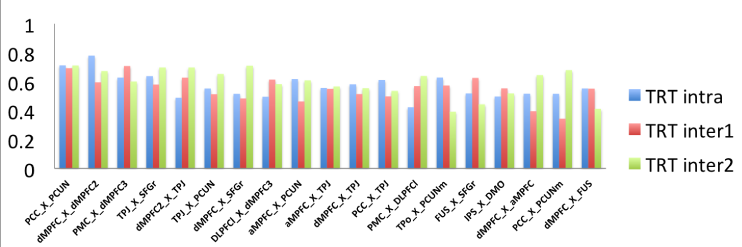
\includegraphics[width=\linewidth]{../figures/fig_icc.png}
\end{center}
\caption[ICC scores]{
  ICC scores for pairs of connections passing the $>0.5$ threshold on the NYU-TRT dataset.
}
\label{fig_icc}
\end{figure}

Average connectivity maps associated with the DMN nodes as well as the nodes outside the DMN that passed the TRT selection are presented in Figures \ref{fig_nodes_DMN} and \ref{fig_nodes_none_DMN}. The involvement of the sensorimotor, visual and attentional networks mainly came from contrasts reporting a decrease of negative correlations in patients, that was interpreted as a compensation mechanism by some authors. These connections are potentially very valuable to monitor the effect of a drug. Considering that we pooled studies of the DMN, we decided to select as candidates all connections of parcels within the DMN, as well as connections between a parcel inside the DMN and a parcel outside the DMN. The final selection of target measures was based on test-retest reliability. All the parcels and associated labels and networks are listed in Table \ref{tab_point-to-point}.


\begin{figure}[H]
\begin{center}
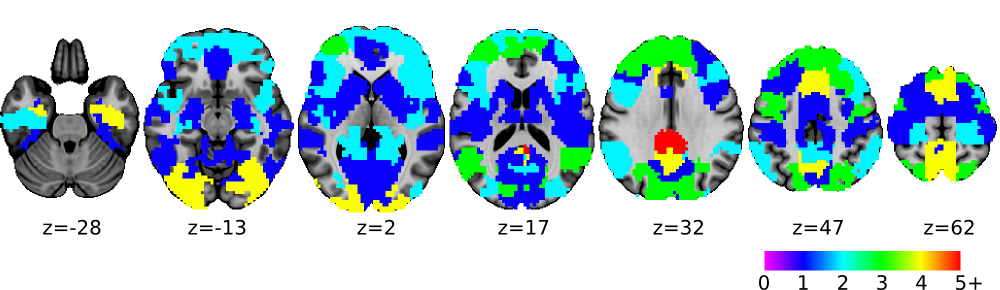
\includegraphics[width=\linewidth]{../figures/fig_freq_sel_dat.png}
\end{center}
\caption[Cited region frequency]{
  Frequency of reported regions showing functional differences based on a literature review of 6 papers.
}
\label{fig_freq_sel}
\end{figure}

\begin{figure}[H]
\begin{center}
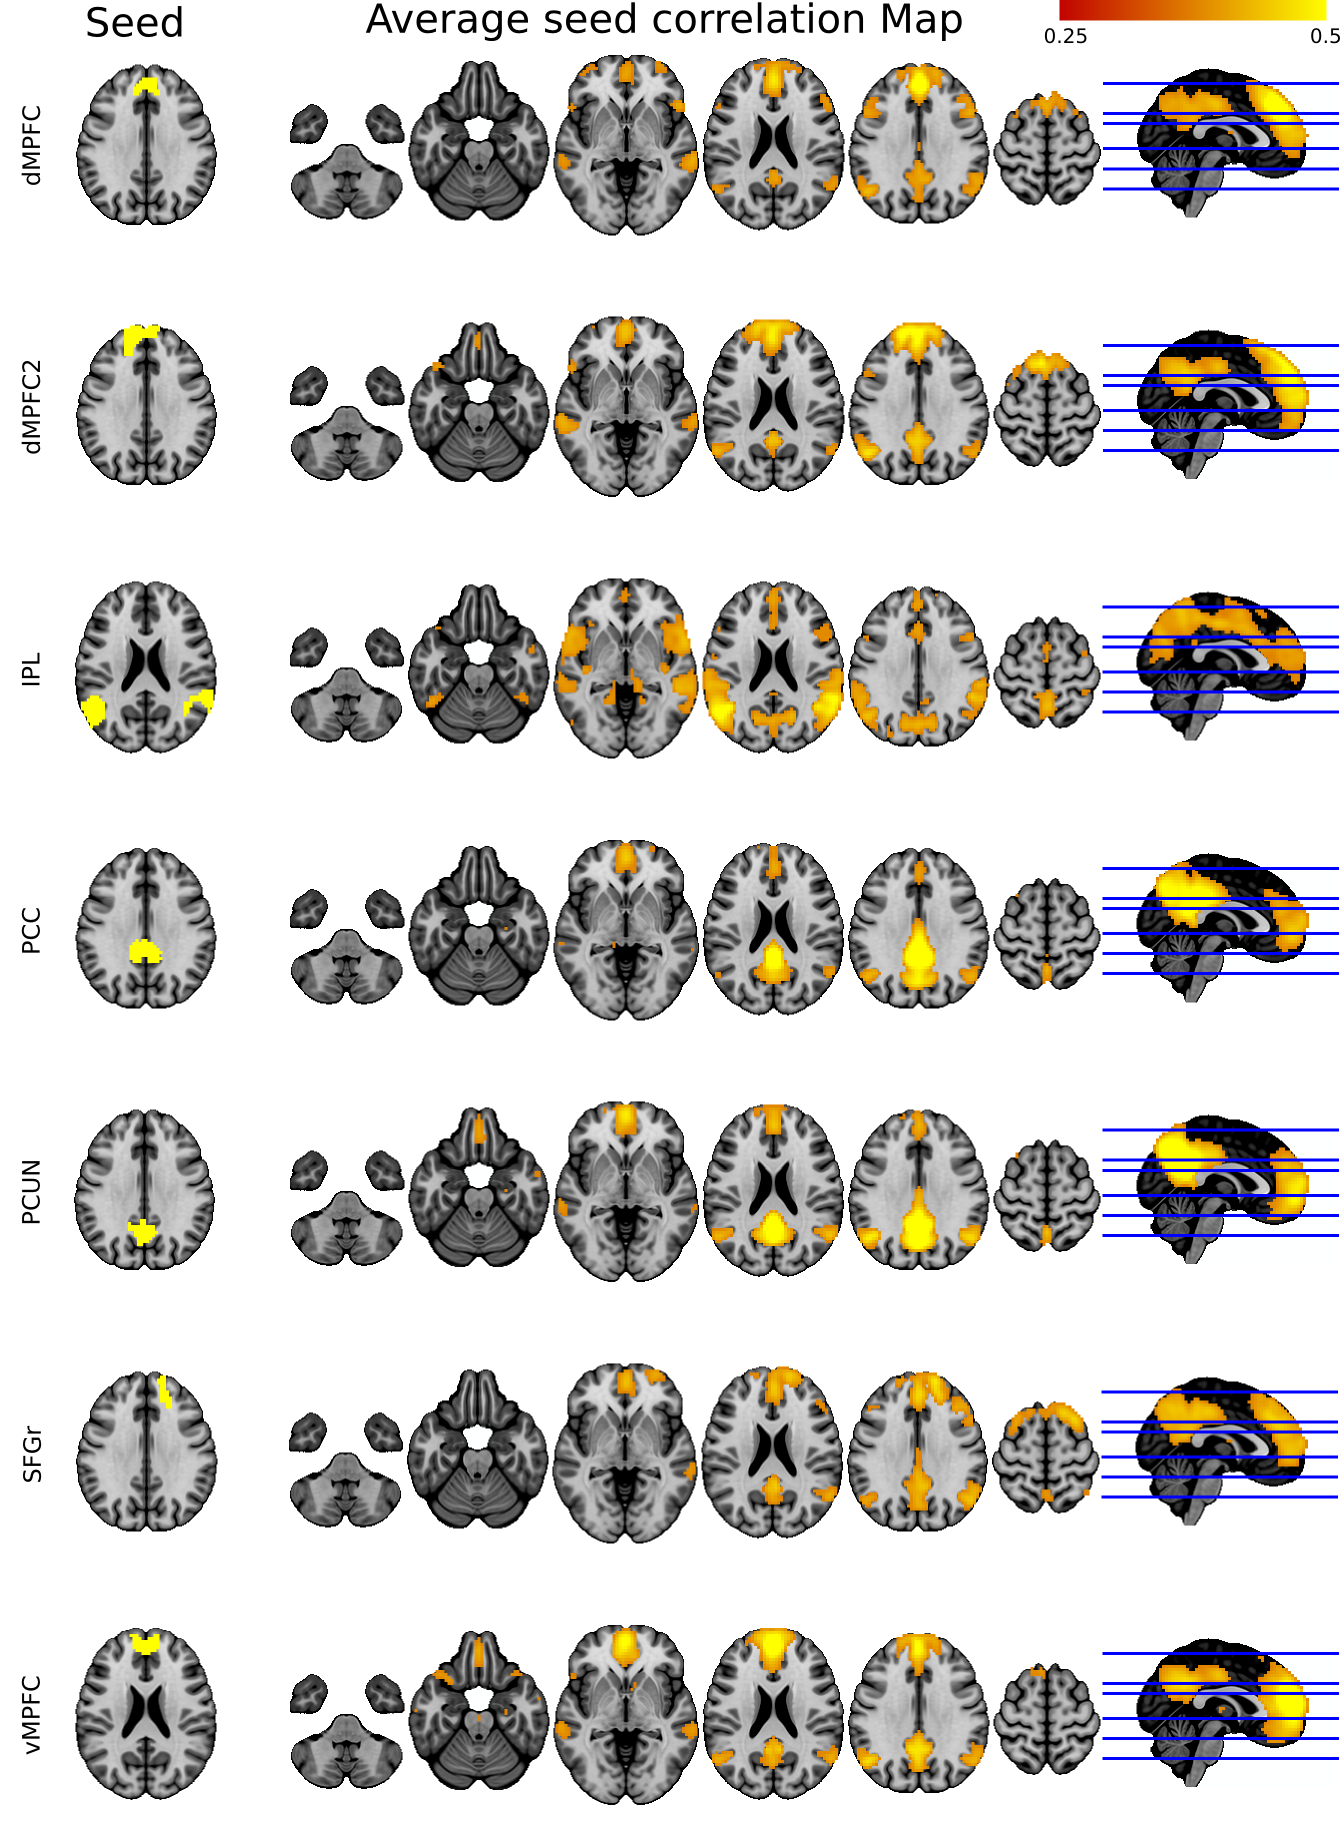
\includegraphics[width=\linewidth]{../figures/fig_nodes_DMN.png}
\end{center}
\caption[Selected region inside DMN]{
  Selected nodes inside the DMN who passed the TRT selection.
}
\label{fig_nodes_DMN}
\end{figure}

\begin{figure}[H]
\begin{center}
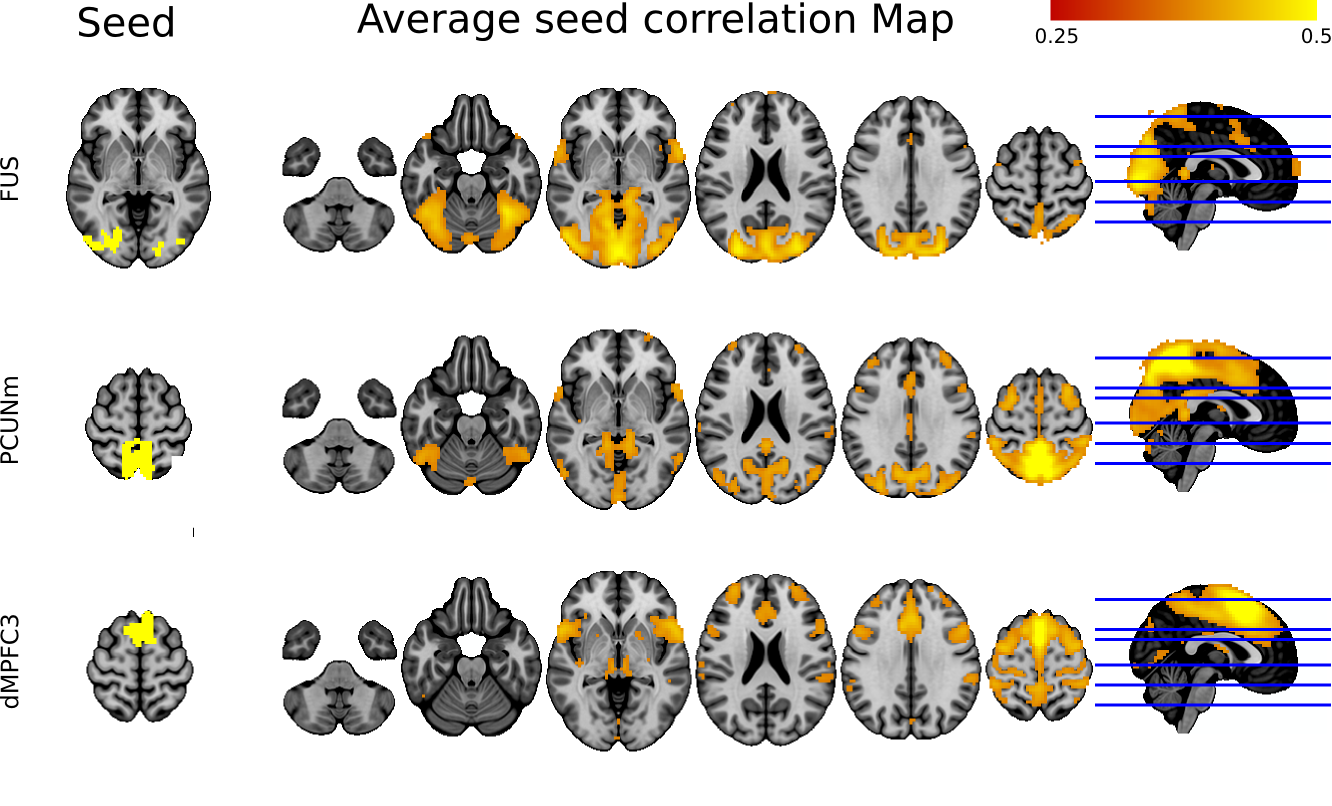
\includegraphics[width=\linewidth]{../figures/fig_nodes_non_DMN.png}
\end{center}
\caption[Selected region outside DMN]{
	  Selected nodes outside the DMN who passed the TRT selection.
}
\label{fig_nodes_none_DMN}
\end{figure}
%Regarding the graph measures, there is a growing arsenal of metrics that have been proposed in the literature, see \citep{Bullmore2009} for a review, notably box 2 for a summary of measures. We selected some of the most standard metrics that have been shown (or suggested) to be impacted by a disease of the Alzheimer type. Regarding local measures, \cite{Buckner2009} noted the similarity of the “degree centrality”, or “hubs” maps in young adults and the patterns of deposition of amyloid-beta in patients suffering of a DAT. This work (or subsequent work as far as we know) did not test directly the relationship between degree centrality and the presence/progress of DAT. An important paper for our purposes is \cite{Supekar2008}, that showed that both local and global clustering coefficients (but not efficiency) are impacted by a DAT. By contrast, \cite{Sanz-Arigita2010} reported that global efficiency (and not global clustering) was impacted by DAT. This inconsistency may simply reflect the low 
%statistical power shared by both studies (18 ECN, 21 patients with mild DAT for the former paper, and 21 ECN, 18 patients with mild DAT for the latter), or methodological differences. Finally, we also included the measure of modularity \citep{Rubinov2011}, a promising tool that has not been used yet in DAT. We used the implementation of the metrics described in \cite{Rubinov2011}. Note that all the metrics first require to binarize the functional connectome of each participant, which was achieved with a density-based threshold (top 20\% positive connections, see the test-retest section below for a rationale).

%In total, the literature review identified 7 nodes in the DMN (21 point-to-point correlations within the DMN) and 9 seeds in networks outside of the DMN (63 point-to-point correlations between a node in the DMN and a node outside of the DMN). We included three local network properties in the DMN (21 measures), as well as two global properties. That's a total of 107 candidate measures, based on a fairly conservative literature review. We further analyzed the test-retest reliability of these measures to narrow the selection down to about 10 measures. 

%The literature on TRT reliability of graph measures is much more difficult to interpret: \cite{Braun2012} for example has included many possible strategies to generate graph properties, resulting into almost the full range of possible ICC values for every metric ! Because no processing strategy was an obvious winner across all metrics, we selected the middle thresholding (20\% density) of \cite{Braun2012}. The relatively low ICC for graph measures (only a few measures with $ICC>0.5$, many measures with $ICC < 0.2$), was consistent with the results of \citep{Wang2011}.

\begin{table}[H]
\begin{center}
\begin{tabular}{l l l l}
\bfseries{Network} & \bfseries{Label} & \bfseries{Name} & \bfseries{Cambridge100}\\
\hline
 & PCC & posterior cingulate cortex & 1\\
 & dMPFC & dorsomedial prefrontal cortex & 12\\
 & dMPFC2 & dorsomedial prefrontal cortex & 46\\
Default-mode network & aMPFC & anterior medial prefrontal cortex & 42\\
 & IPL & inferior parietal lobule & 49\\
 & PCUN & precuneus & 53\\
 & MTL & medial temporal lobe & 39\\
 & SFGr & right superior frontal gyrus & 76\\
\hline
Visual network & FUS & fusiformgyrus & 71\\
\hline
Dorsal attentional & PCUMm & precuneus (motor) & 94\\
\hline
Cingulo-opercular network & dMPFC3 & dorsmedial prefrontal cortex & 90\\
\end{tabular}
\end{center}
\caption{Regions selected in the literature review, the region number correspond to the number in the Cambridge 100 partition.}
\label{tab_point-to-point}
\end{table}

For point-to-point correlations within the DMN, we selected the connections with highest ICC for each node (all average ICC > 0.5):
\begin{itemize}
\item PCC x PCUN
\item dMPFC x dMPFC2
\item IPL x SFGr
\item aMPFC x PCUN
\end{itemize}
For each point-to-point correlation between the DMN and another network, we selected the connections with highest ICC and ICC > 0.5:
\begin{itemize}
\item FUS x SFGr
\item PCC x PCUNm
\item IPL x dMPFC3
\end{itemize}
% The only graph properties that satisfied the above criteria were:
% \begin{itemize}
% \item[•] average clustering
% \item[•] clustering PCUN
% \item[•] local efficiency PCUN
% \end{itemize}


The first assessment perform on the dataset was to verify the distribution of the variance in functional connectivity among each site and across sites in order to see if they are of the same order of magnitude or not. This analysis of Figure \ref{fig_site_variability} shows the distribution of the standard deviation of connectivity across subjects (the distribution is over the full brain connectome, with several 1000s connections) at the 8 sites against the inter-sites standard deviation of connectomes (average at each site). as we can see the inter-site (between site) variability is smaller than the intra-site (between subjects) variability.

\begin{figure}[H]
\begin{center}
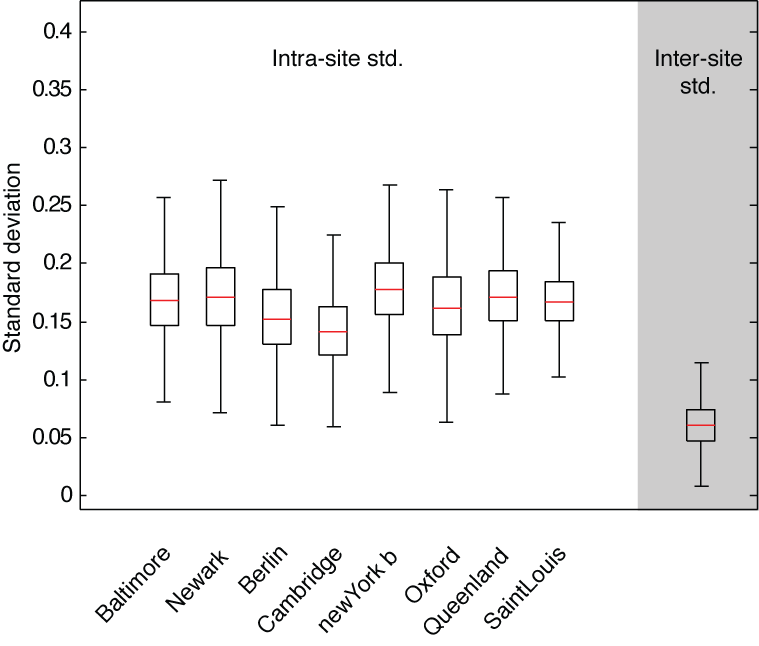
\includegraphics[width=\linewidth]{../figures/inter_vs_intra_3tonly.png}
\end{center}
\caption[inter vs. intra site variability]{
  Distribution of intra-site (between-subject) standard deviation vs. inter-site (between-site) standard deviation, based on the standard deviation of the connectivity matrices from 8 sites from the 1000 functional connectome dataset.
}
\label{fig_site_variability}
\end{figure}

In order to verify how spatial structure vary across sites the average standard deviation and the average connectivity map of the DMN was extracted for each site and displayed in Figure \ref{fig_DMN_variability}. In order to ease the reading we selected only 4 representative sites, although we reached the same conclusion on all the sites. As we can see in the intersection between two sites the difference in standard deviation between-sites was illustrated (red set of brain cuts). First the mean DMN at each site is consistent with the expected spatial ditribution reported in other studies. As we can see the amplitude of inter-site bias is about 3-fold smaller than the within-site standard deviation (red \textasciitilde0.06 vs. orange \textasciitilde0.18). The most salient changes between-sites are located in the mesio-frontal region associated with the anterior part of the DMN. This last finding may be associated with motion artefact as previously reported in \cite{Dansereau2014}.



\begin{figure}[H]
\begin{center}
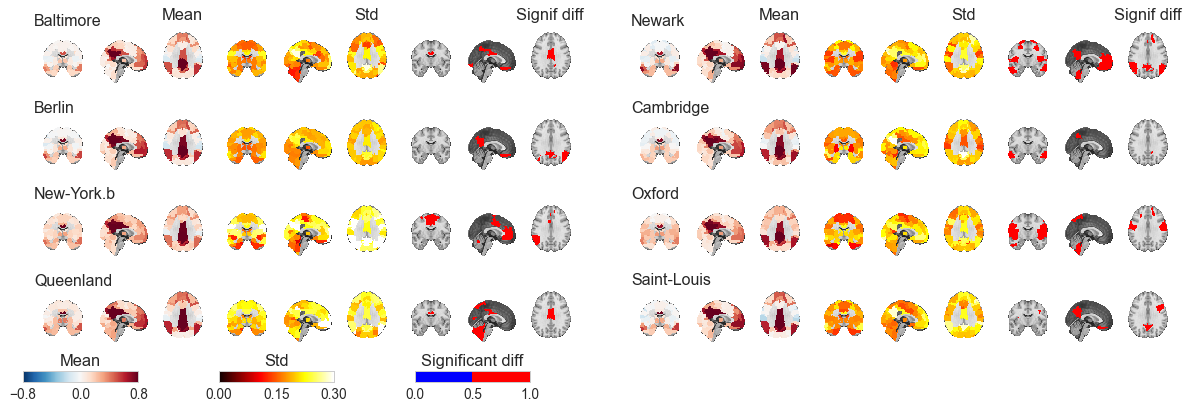
\includegraphics[width=\linewidth]{../figures/pccmap_multisite.png}
\end{center}
\caption[DMN variability across sites]{
Functional connectivity maps of the default-mode network at multiple sites. The average connectivity map for 4 sites (Baltimore, Cambridge, Newark and New-Yorkb at 3T) are presented on the diagonal (left). The standard deviation across subjects and within site is presented next to it (diagonal squares, right part). Each off-diagonal block represent the absolute difference between the average functional connectivity maps between two sites (called the inter-site bias).
}
\label{fig_DMN_variability}
\end{figure}


\begin{figure}[H]
\begin{center}
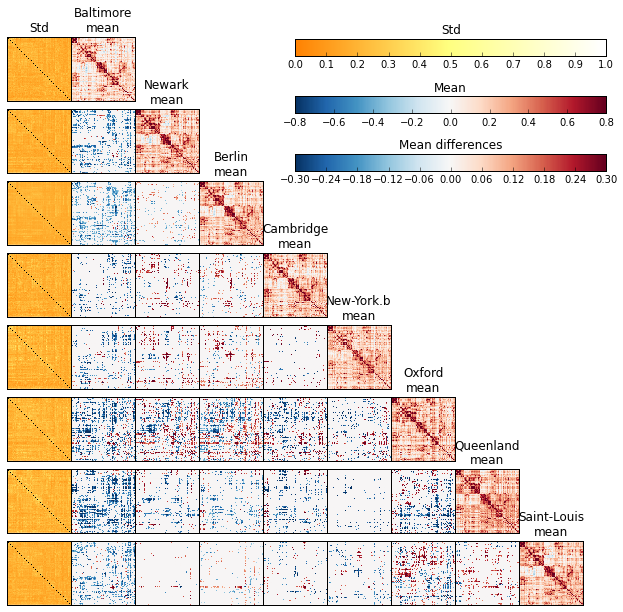
\includegraphics[width=\linewidth]{../figures/connectome_multisite.png}
\end{center}
\caption[Connectome variability across sites]{
Functional connectome for multiple sites. The average connectome of 7 sites (Baltimore, Cambridge, Newark and New-Yorkb, Oxford, Queenland, SaintLouis at 3T) are presented on the diagonal (left). The standard deviation across subjects and within site is presented next to it (diagonal squares, right part). Each off-diagonal block represent the absolute difference between the average functional connectivity maps between two sites (called the inter-site bias).
}
\label{fig_DMN_variability}
\end{figure}


We also showed using Monte-Carlo simulations that the power of detecting an effect is marginally affected by the site acquisition configuration (single site or multi-site, see Figure3.2 for an illustration of a power analysis on three different seeds) where the sites are balanced in term of the amount of subject with and without the effect. 

\begin{figure}[H]
\begin{center}
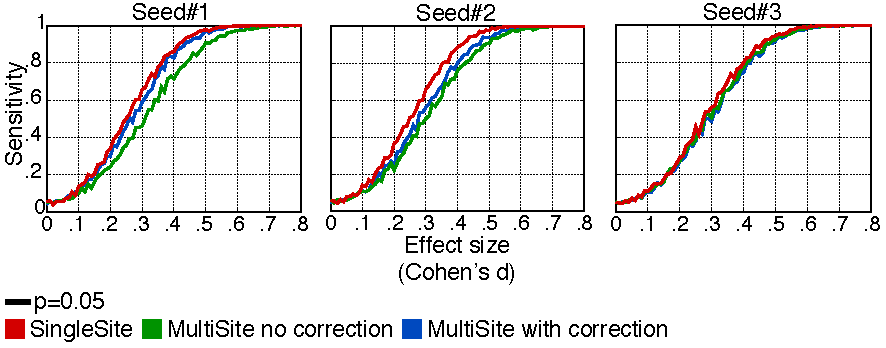
\includegraphics[width=\linewidth]{../figures/simu_results_multisite.pdf}
\end{center}
\caption[Detection power]{
Power analysis for a resting-state fMRI study. A Monte-Carlo simulation was implemented to evaluate the power of a resting-state multi-site study, based on real values of three connections in the default-mode network PCC/MFC, rHIP/vMFC and lIPC-rDLPFC. For each site and each sample, half of the subjects were randomly assigned to a 'treatment' group. For the subjects in this group, a value was added to achieve a given relative effect size (Cohen's d, i.e. the mean of the two groups divided by the standard deviation of all sites). The significance of the difference between the control and 'treatment' group was assessed by a $t$-test in a linear model, including covariates to model site-specific bias. The study was repeated for various effect sizes (0 to 0.8 with a step of 0.01) at a threshold of 0.05 on the p-value in the $t$-test. For a p of 0.05, a statistical power of 0.
95 can be achieved for as low as a 0.47 effect size. The simulation was based on a scenario with 8 sites and 385 subjects, and no homogeneization of acquisition protocol whatsoever. The multi-site (with and without correction) is based on 187 subjects from 7 sites and the SingleSite is based on one site of 198 subjects. 
}
\label{fig_detection_power}
\end{figure}

\begin{figure}[H]
\begin{center}
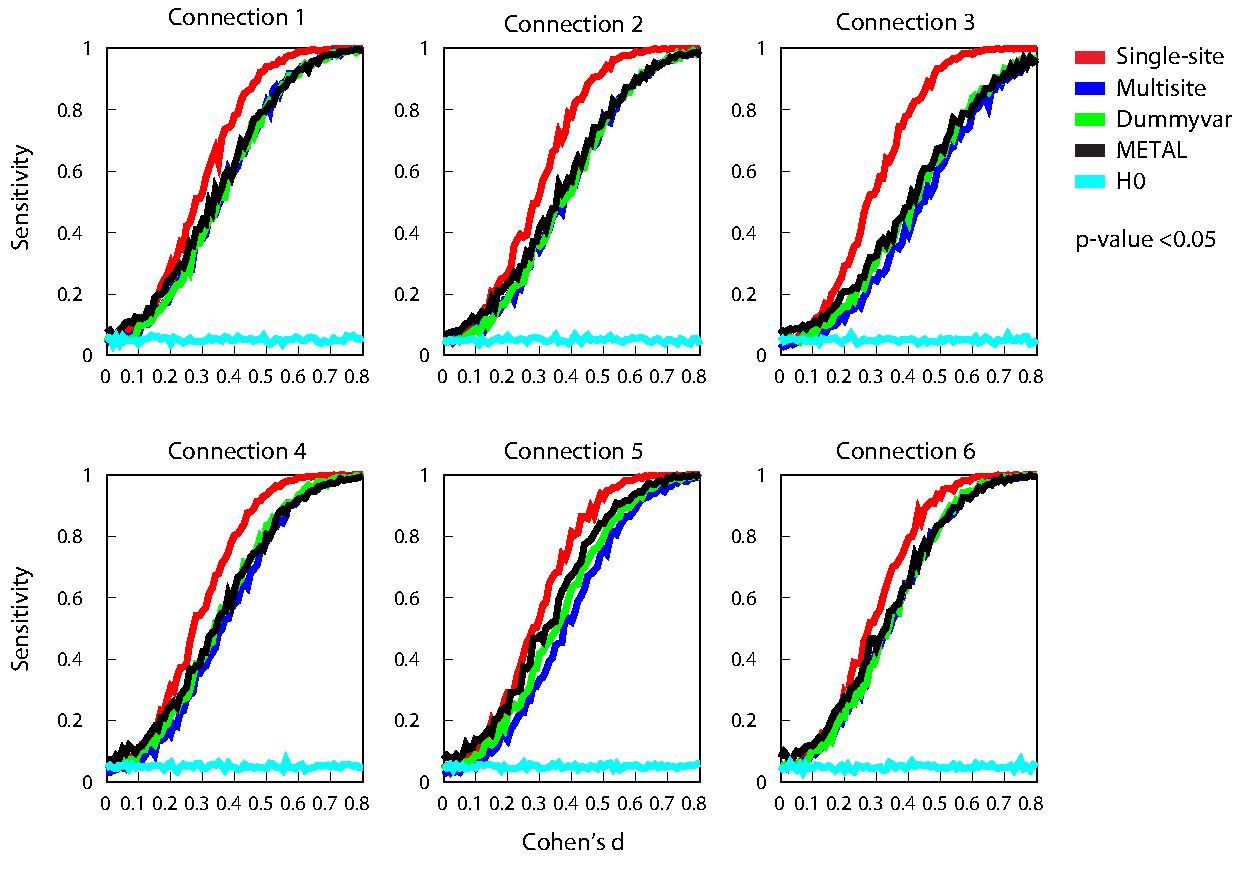
\includegraphics[width=\linewidth]{../figures/multisite_simulation_50pct.pdf}
\end{center}
\caption[Detection power 2]{
Power analysis for a resting-state fMRI study. A Monte-Carlo simulation was implemented to evaluate the power of a resting-state multi-site study. For each site and each sample, half of the subjects were randomly assigned to a 'treatment' group. For the subjects in this group, a value was added to achieve a given relative effect size (Cohen's d, i.e. the mean of the two groups divided by the standard deviation of all sites). The significance of the difference between the control and 'treatment' group was assessed by a $t$-test in a linear model. To correct for site-specific bias two correction are presented the dummy variables and METAL. The study was repeated for various effect sizes (0 to 0.8 with a step of 0.01) at a threshold of 0.05 on the p-value in the $t$-test. The simulation was based on a scenario with 8 sites and 385 subjects, and no homogeneization of acquisition protocol whatsoever. The multi-site (with and without correction) is based on 187 subjects from 7 sites and the Single-site is based on 
one site of 198 subjects. 
}
\label{fig_simu_50pct}
\end{figure}

\begin{figure}
\begin{center}
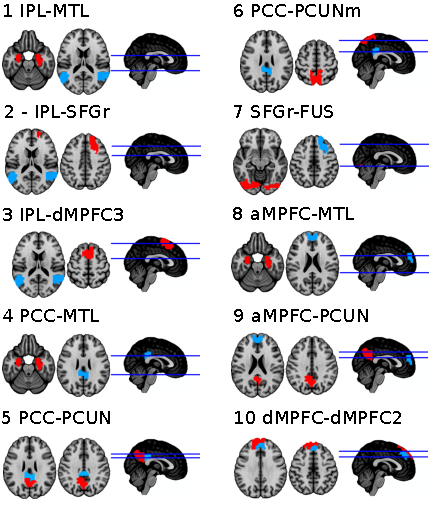
\includegraphics[width=0.5\linewidth]{../figures/p2p_seeds.pdf}
\end{center}
\tiny{Connexions pair based on a literature review}
\label{fig_p2p}
\end{figure}


\begin{figure*}
        \centering
        \begin{subfigure}[b]{0.31\textwidth}
            \centering
            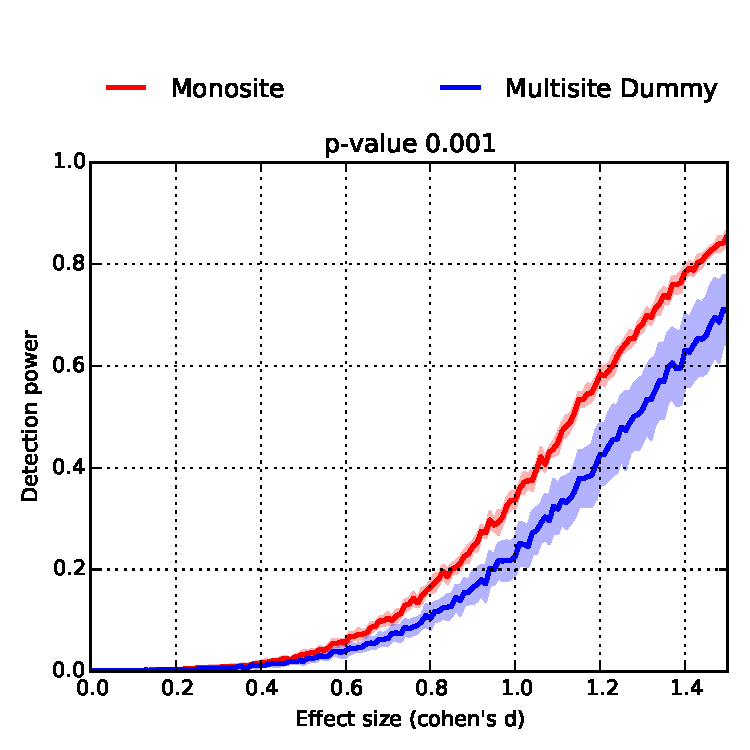
\includegraphics[width=\textwidth]{../figures/realdata_detect_pow_s40_50pct.pdf}
            %\caption[]%
            {{\tiny 40 subjects}}    
            \label{fig:mean and std of net14}
        \end{subfigure}
        \hfill
        \begin{subfigure}[b]{0.31\textwidth}  
            \centering 
            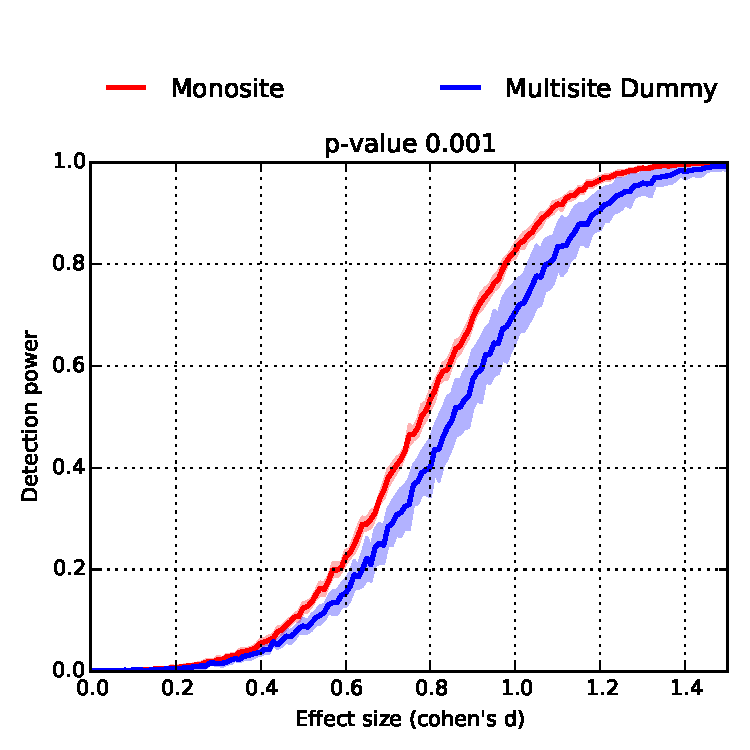
\includegraphics[width=\textwidth]{../figures/realdata_detect_pow_s80_50pct.pdf}
            %\caption[]%
            {{\tiny 80 subjects}}    
            \label{fig:mean and std of net24}
        \end{subfigure}
        \hfill
        \begin{subfigure}[b]{0.31\textwidth}   
            \centering 
            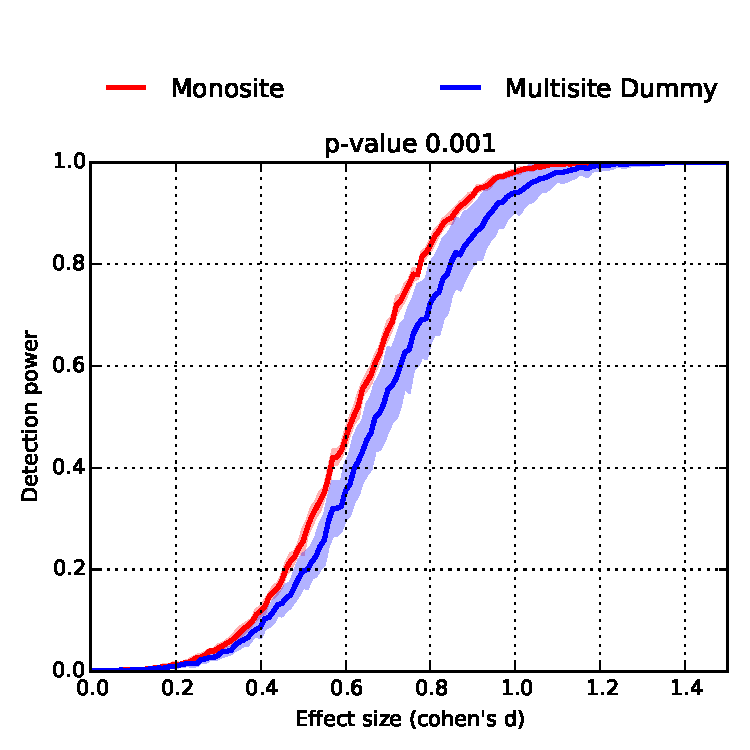
\includegraphics[width=\textwidth]{../figures/realdata_detect_pow_s120_50pct.pdf}
            %\caption[]%
            {{\tiny 120 subjects}}    
            \label{fig:mean and std of net34}
        \end{subfigure}
        \caption[]
        {\small Simulation on real data of the detection power of two groups balanced 50\%-50\% between 7 sites. All plot show four scenario, one monosite, 7 sites with no correction for differences in variability between sites, 7 sites with correction for multisite differences using dummy variables and 7 sites with correction for multisite differences using METAL weighted average. Each plot show the detection power in function of the effect size for 3 different sample size 40, 80 and 120 subjects in total.} 
        \label{fig:real_sim_samplesize_5050}
    \end{figure*}
    
    
\begin{figure*}
        \centering
        \begin{subfigure}[b]{0.31\textwidth}
            \centering
            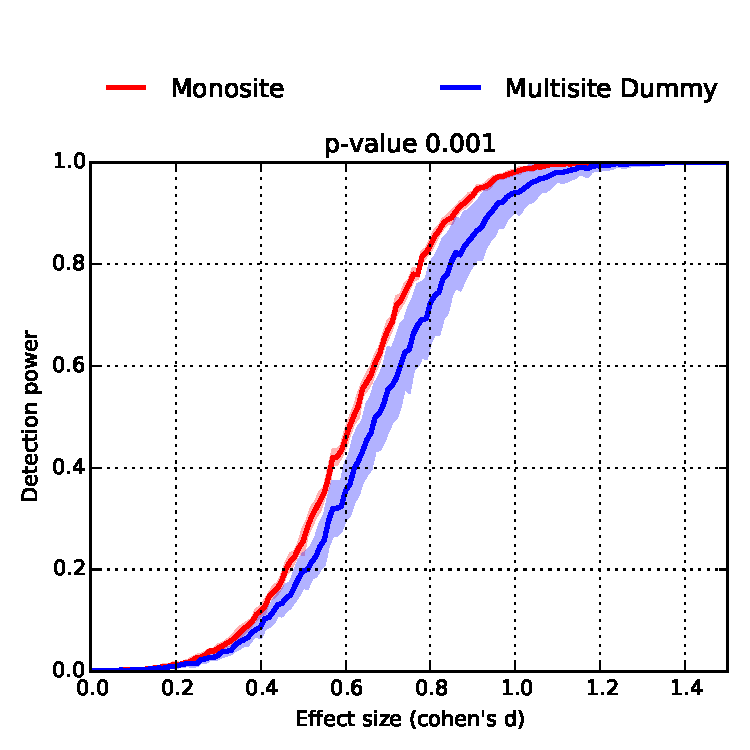
\includegraphics[width=\textwidth]{../figures/realdata_detect_pow_s120_50pct.pdf}
            %\caption[]%
            {{\tiny balancing 50\%}}    
            \label{fig:mean and std of net14}
        \end{subfigure}
        \hfill
        \begin{subfigure}[b]{0.31\textwidth}  
            \centering 
            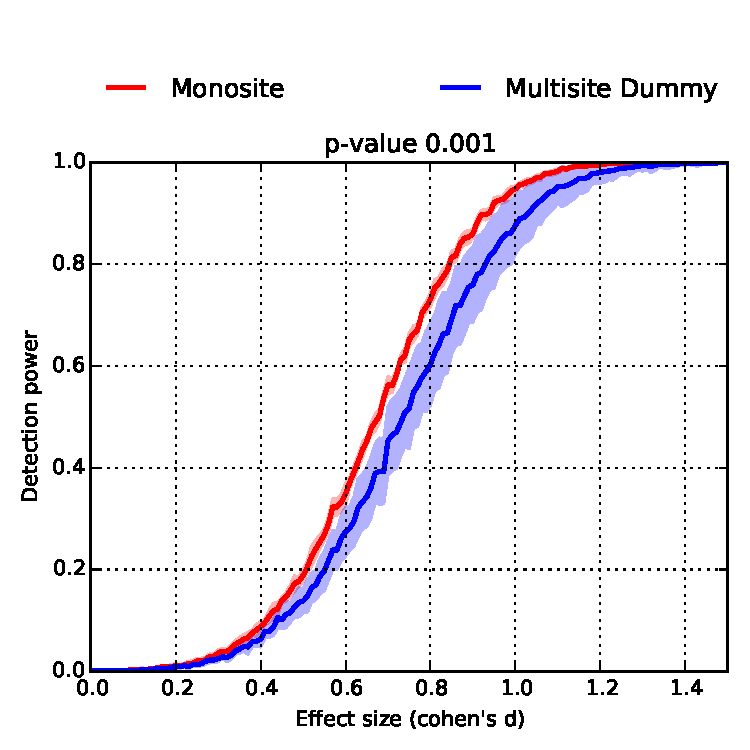
\includegraphics[width=\textwidth]{../figures/realdata_detect_pow_s120_30pct.pdf}
            %\caption[]%
            {{\tiny balancing 30\%}}    
            \label{fig:mean and std of net24}
        \end{subfigure}
        \hfill
        \begin{subfigure}[b]{0.31\textwidth}   
            \centering 
            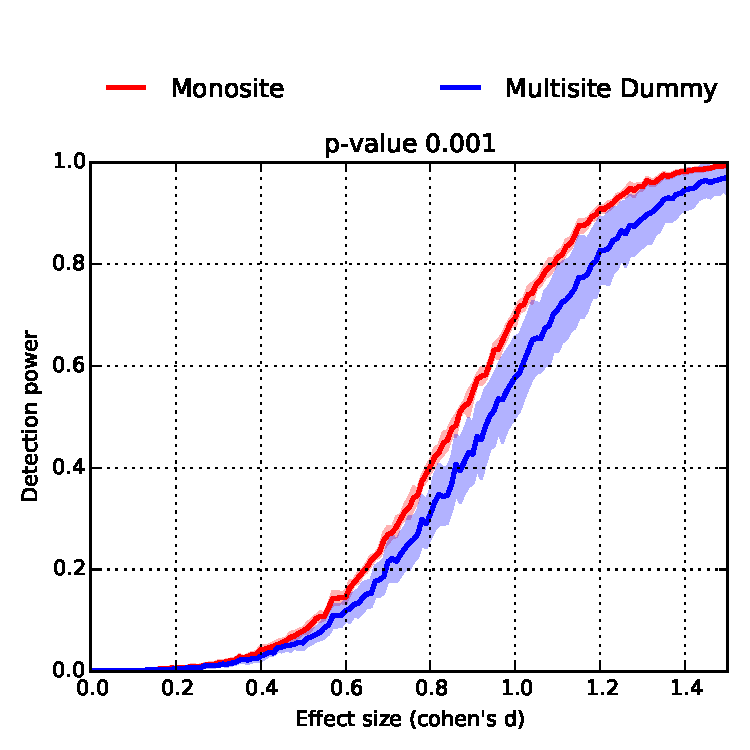
\includegraphics[width=\textwidth]{../figures/realdata_detect_pow_s120_15pct.pdf}
            %\caption[]%
            {{\tiny balancing 15\%}}    
            \label{fig:mean and std of net34}
        \end{subfigure}
        \caption[]
        {\small Simulation on real data of the detection power of two groups for a total of 120 subject between 7 sites. All plot show four scenario, one monosite, 7 sites with no correction for differences in variability between sites, 7 sites with correction for multisite differences using dummy variables and 7 sites with correction for multisite differences using METAL weighted average.} 
        \label{fig:real_sim_samplesize_varbalancing}
    \end{figure*}
    
\begin{figure*}
        \centering
        \begin{subfigure}[b]{0.31\textwidth}
            \centering
            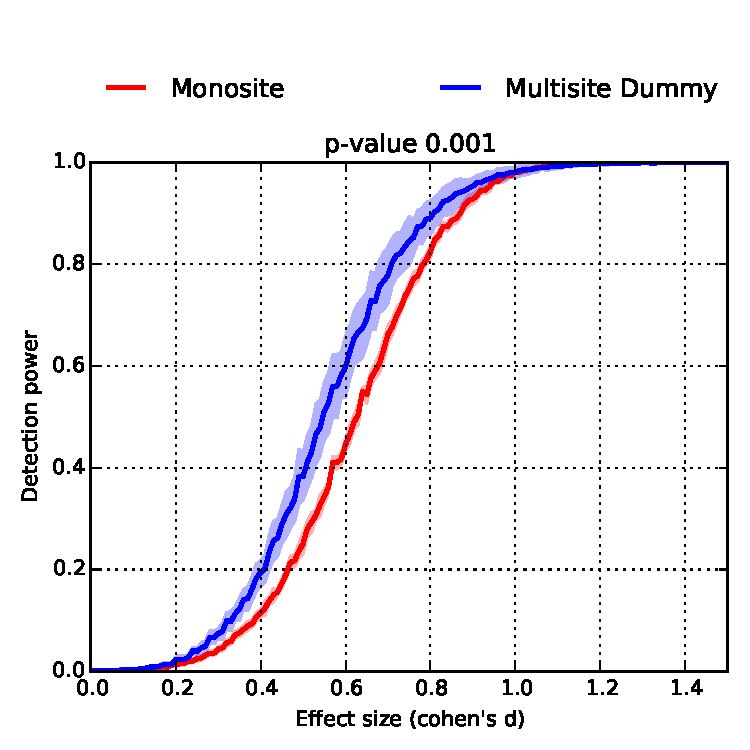
\includegraphics[width=\textwidth]{../figures/realdata_detect_pow_sitepatho_s120_50pct.pdf}
            %\caption[]%
            {{\tiny balancing 50\%}}    
            \label{fig:mean and std of net14}
        \end{subfigure}
        \hfill
        \begin{subfigure}[b]{0.31\textwidth}  
            \centering 
            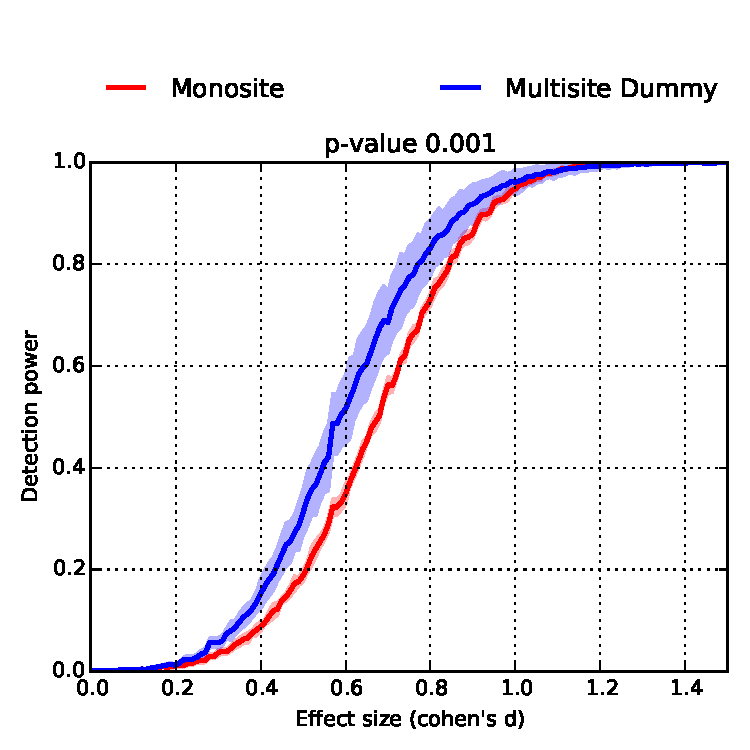
\includegraphics[width=\textwidth]{../figures/realdata_detect_pow_sitepatho_s120_30pct.pdf}
            %\caption[]%
            {{\tiny balancing 30\%}}    
            \label{fig:mean and std of net24}
        \end{subfigure}
        \hfill
        \begin{subfigure}[b]{0.31\textwidth}   
            \centering 
            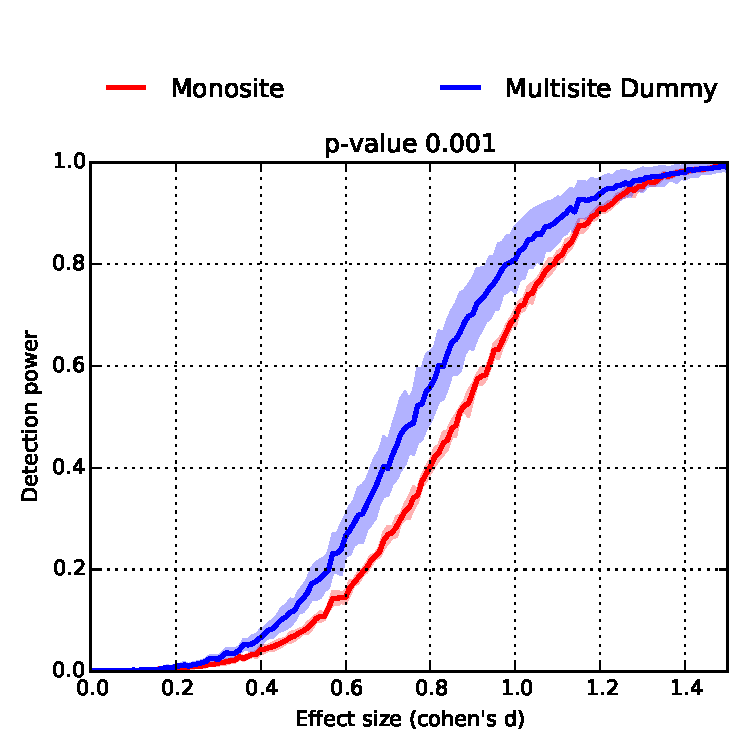
\includegraphics[width=\textwidth]{../figures/realdata_detect_pow_sitepatho_s120_15pct.pdf}
            %\caption[]%
            {{\tiny balancing 15\%}}    
            \label{fig:mean and std of net34}
        \end{subfigure}
        \caption[]
        {\small Simulation on real data of the detection power of two groups for a total of 120 subject between 7 sites. All plot show four scenario, one monosite, 7 sites with no correction for differences in variability between sites, 7 sites with correction for multisite differences using dummy variables and 7 sites with correction for multisite differences using METAL weighted average.}
         
        \label{fig:real_sim_samplesize_5050}
\end{figure*}
    
\begin{figure*}
        \centering
        \begin{subfigure}[b]{0.475\textwidth}
            \centering
            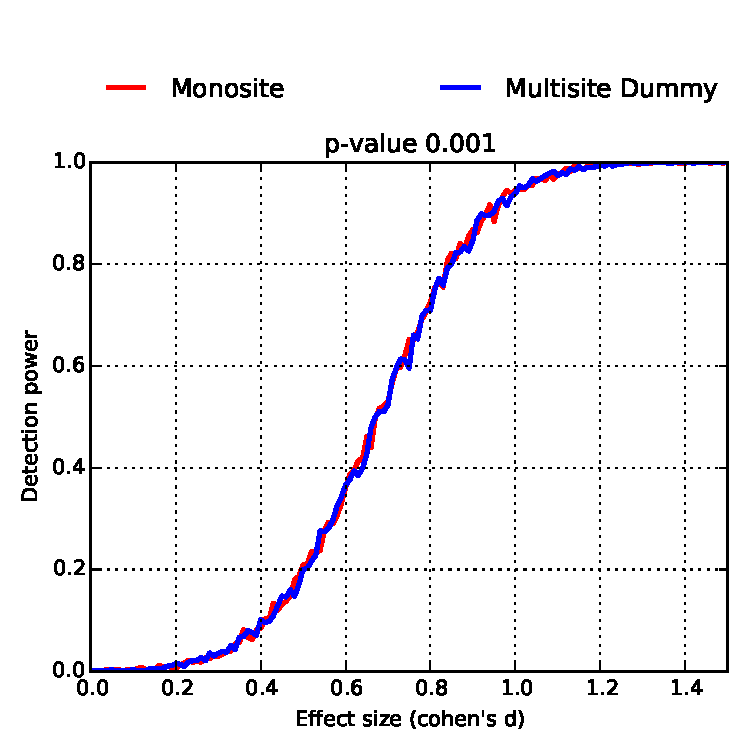
\includegraphics[width=\textwidth]{../figures/detect_pow_bal5050_var0_site0.pdf}
            %\caption[]% 
            {{\tiny No site effect}}    
            \label{fig:mean and std of net14}
        \end{subfigure}
        \hfill
        \begin{subfigure}[b]{0.475\textwidth}  
            \centering 
            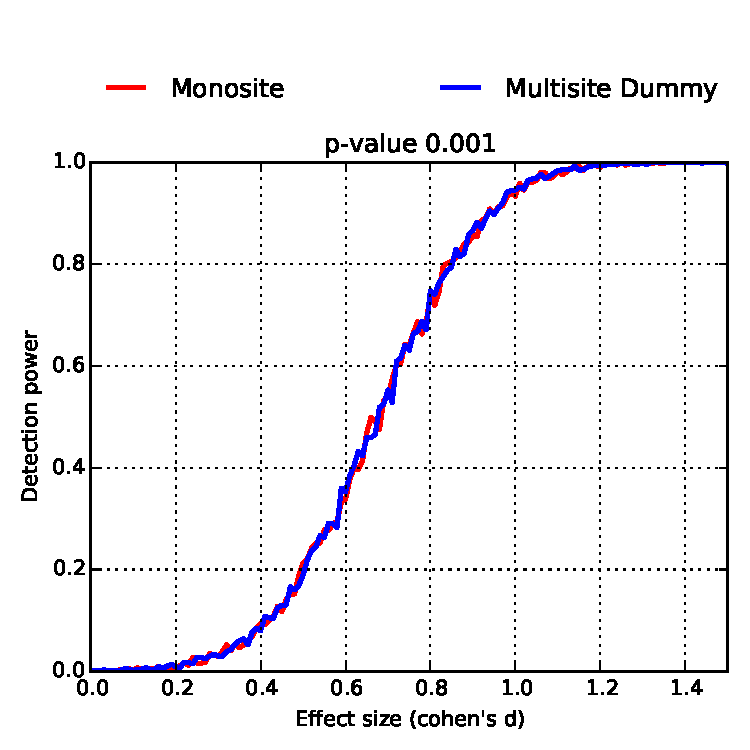
\includegraphics[width=\textwidth]{../figures/detect_pow_bal5050_var0_site05.pdf}
            %\caption[]%
            {{\tiny Site effect of 0.5}}    
            \label{fig:mean and std of net24}
        \end{subfigure}
        \vskip\baselineskip
        \begin{subfigure}[b]{0.475\textwidth}   
            \centering 
            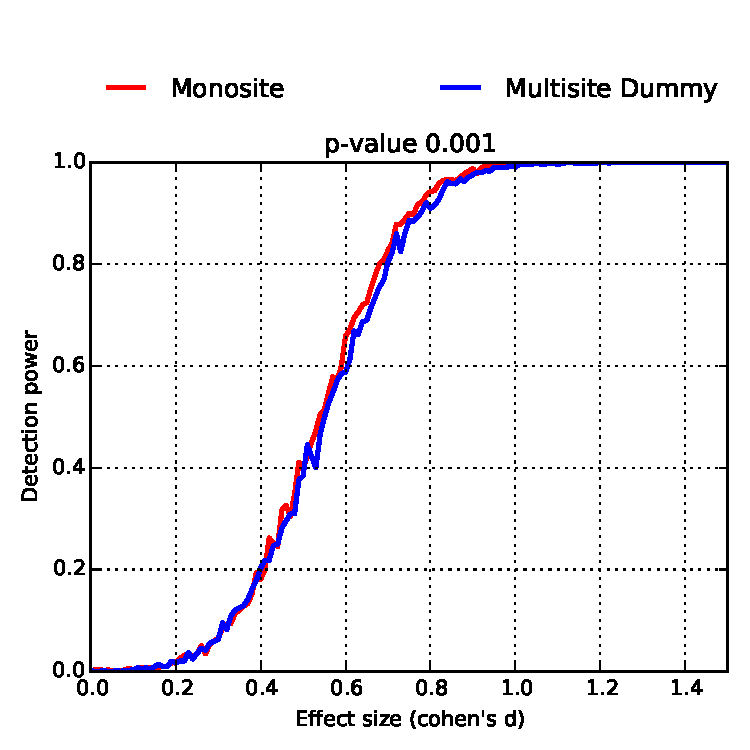
\includegraphics[width=\textwidth]{../figures/detect_pow_bal5050_var2_site0.pdf}
            %\caption[]%
            {{\tiny Patho effect in function of site}}    
            \label{fig:mean and std of net34}
        \end{subfigure}
        \quad
        \begin{subfigure}[b]{0.475\textwidth}   
            \centering 
            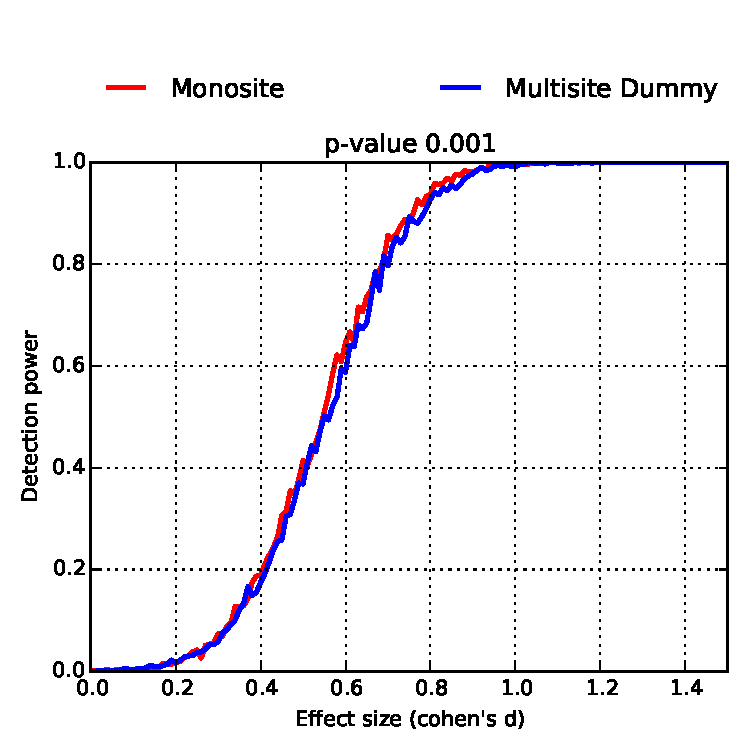
\includegraphics[width=\textwidth]{../figures/detect_pow_bal5050_var2_site05.pdf}
            %\caption[]%
            {{\tiny Patho effect in function of site + site effect}}    
            \label{fig:mean and std of net44}
        \end{subfigure}
        \caption[]
        {\small Simulation of the detection power of two groups balanced 50\%-50\% between two sites. All plot show four scenario, one monosite, two sites with no correction for differences in variability between sites, two sites with correction for multisite differences using dummy variables and two sites with correction for multisite differences using METAL weighted average. The plots show the detection power when the variability is greater in one side then the other for the pathology group (twice the reference variability in one site and half the reference variability in the other one)} 
        \label{fig:sim_5050}
    \end{figure*}
    
    
    
\begin{figure*}
        \centering
        \begin{subfigure}[b]{0.475\textwidth}
            \centering
            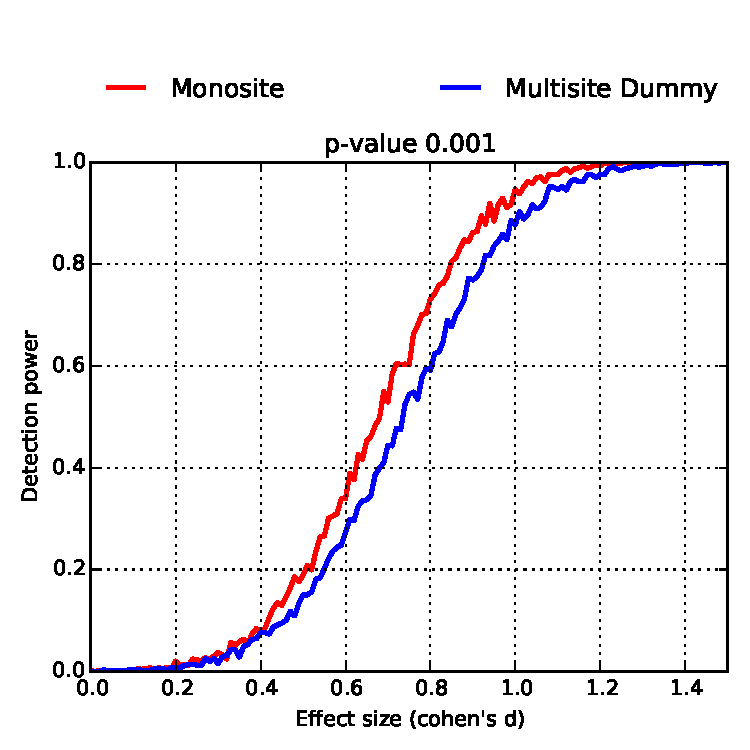
\includegraphics[width=\textwidth]{../figures/detect_pow_bal7030_var0_site0.pdf}
            %\caption[]%
            {{\tiny No site effect}}    
            \label{fig:mean and std of net14}
        \end{subfigure}
        \hfill
        \begin{subfigure}[b]{0.475\textwidth}  
            \centering 
            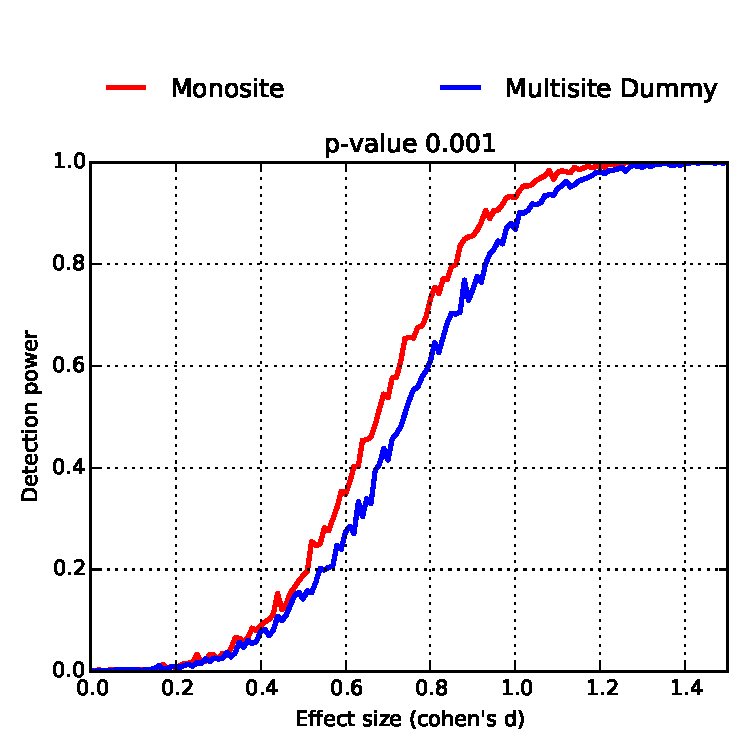
\includegraphics[width=\textwidth]{../figures/detect_pow_bal7030_var0_site05.pdf}
            %\caption[]%
            {{\tiny Site effect of 0.5}}    
            \label{fig:mean and std of net24}
        \end{subfigure}
        \vskip\baselineskip
        \begin{subfigure}[b]{0.475\textwidth}   
            \centering 
            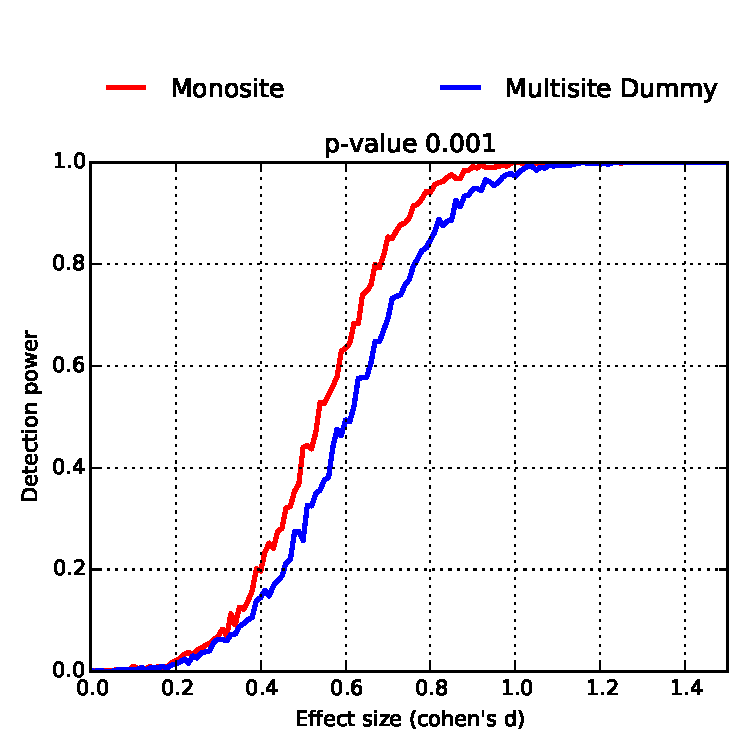
\includegraphics[width=\textwidth]{../figures/detect_pow_bal7030_var2_site0.pdf}
            %\caption[]%
            {{\tiny Patho effect in function of site}}    
            \label{fig:mean and std of net34}
        \end{subfigure}
        \quad
        \begin{subfigure}[b]{0.475\textwidth}   
            \centering 
            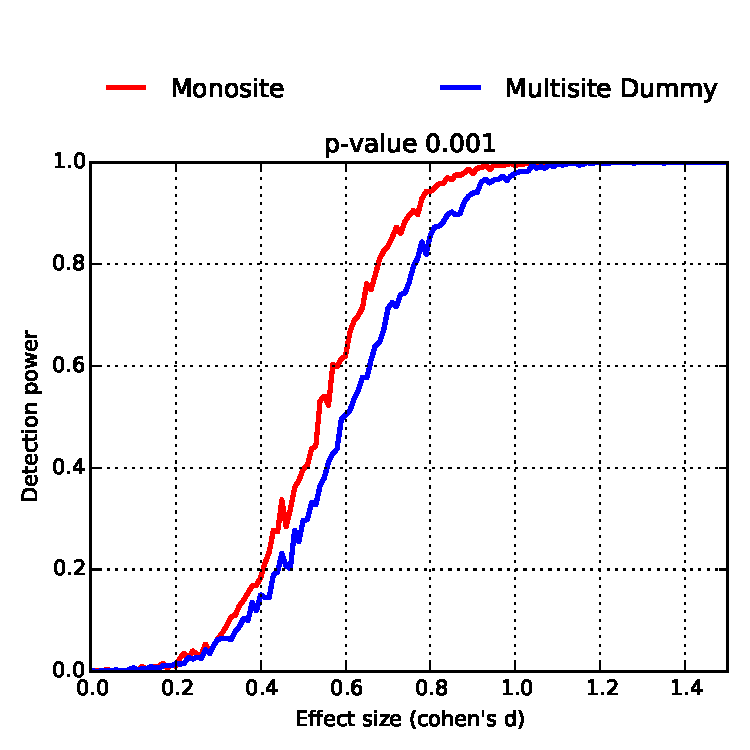
\includegraphics[width=\textwidth]{../figures/detect_pow_bal7030_var2_site05.pdf}
            %\caption[]%
            {{\tiny Patho effect in function of site + site effect}}    
            \label{fig:mean and std of net44}
        \end{subfigure}
        \caption[]
        {\small balance 70\%-30\%} 
        \label{fig:mean and std of nets}
    \end{figure*}
    
    
\begin{figure*}
        \centering
        \begin{subfigure}[b]{0.475\textwidth}
            \centering
            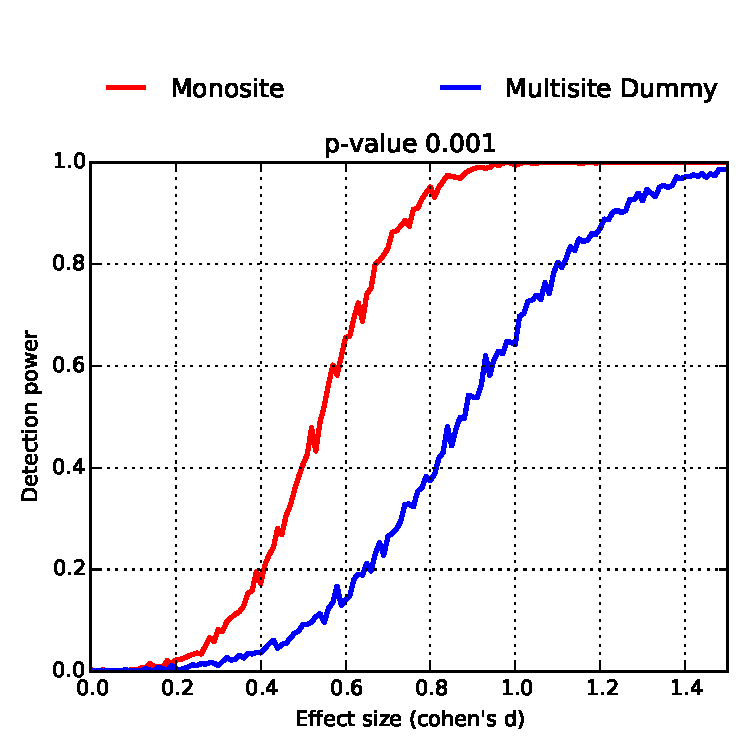
\includegraphics[width=\textwidth]{../figures/detect_pow_2080bal5050_var2_site0.pdf}
            %\caption[]%
            {\tiny{ Patho effect in function of site}}    
            \label{fig:2080 bal5050 var2 site0}
        \end{subfigure}
        \hfill
        \begin{subfigure}[b]{0.475\textwidth}  
            \centering 
            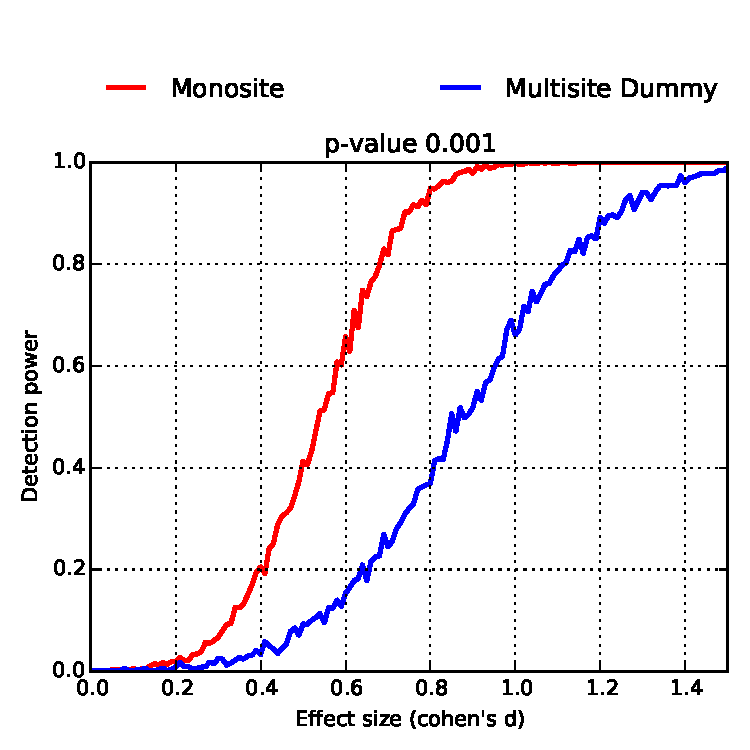
\includegraphics[width=\textwidth]{../figures/detect_pow_2080bal5050_var2_site05.pdf}
            %\caption[]%
            {{\tiny Patho effect in function of site + site effect}}    
            \label{fig:2080 bal5050 var2 site05}
        \end{subfigure}
        \caption[]
        {\small Small and big site, balance 50\%-50\%} 
        \label{fig:mean and std of nets}
    \end{figure*}


\begin{figure*}
        \centering
        \begin{subfigure}[b]{0.475\textwidth}
            \centering
            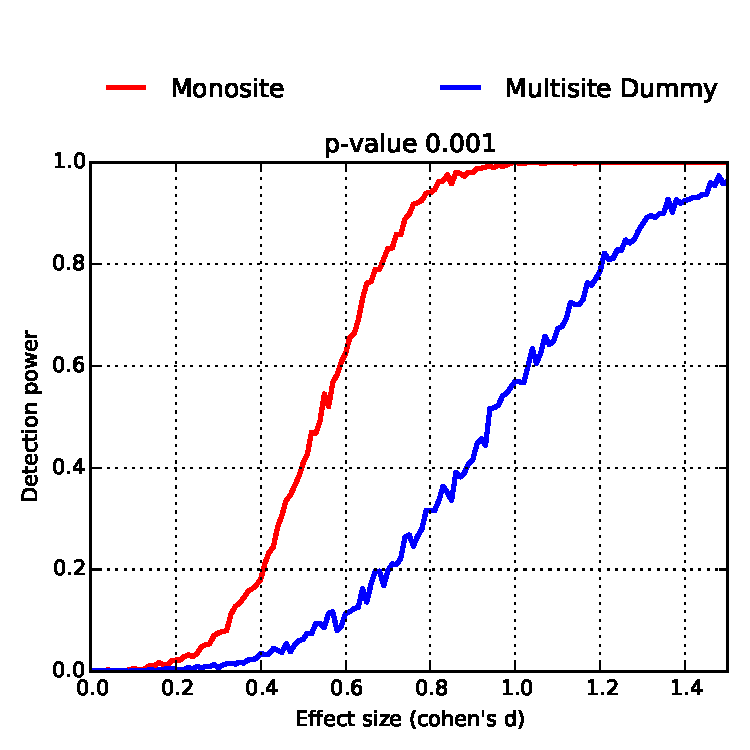
\includegraphics[width=\textwidth]{../figures/detect_pow_2080bal7030_var2_site0.pdf}
            %\caption[]%
            {\tiny{ Patho effect in function of site}}    
            \label{fig:2080 bal7030 var2 site0}
        \end{subfigure}
        \hfill
        \begin{subfigure}[b]{0.475\textwidth}  
            \centering 
            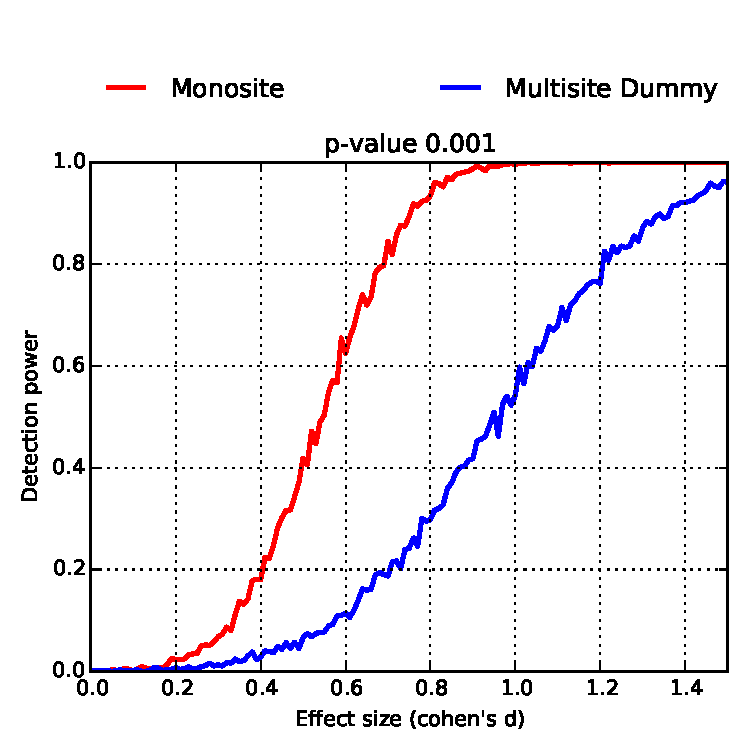
\includegraphics[width=\textwidth]{../figures/detect_pow_2080bal7030_var2_site05.pdf}
            %\caption[]%
            {{\tiny Patho effect in function of site + site effect}}    
            \label{fig:2080 bal7030 var2 site05}
        \end{subfigure}
        \caption[]
        {\small Small and big site, balance 70\%-30\%} 
        \label{fig:mean and std of nets}
    \end{figure*}

\section{Conclusion}

We confirmed that multi-site acquisition introduce some variability in the dataset although a single-site study with 200 subjects had only a marginally superior statistical power than an analysis pooling 7 sites for an equivalent number of subjects, see Figure \ref{fig_detection_power}. In both cases, a high sensitivity ($>0.95$) could be achieved for the effect size observed by \cite{Goveas2011} which reported an effect equivalent to 1. We can therefore conclude that it is feasible to acquire rs-fMRI data in across multiple sites and correct for this topology.





\section{Acknowledgments}
Parts of this work were presented at the 2013 annual meetings of the organization for human brain mapping \citep{Dansereau2013}, as well as the  Alzheimer's Association International Conference (AAIC) (2014) (Copenhagen) \citep{Dansereau2014}. The authors are grateful to the members of the 1000 functional connectome consortium for publicly releasing there dataset. The computational resources used to perform the data analysis were provided by ComputeCanada\footnote{\url{https://computecanada.org/}} and CLUMEQ\footnote{\url{http://www.clumeq.mcgill.ca/}}, which is funded in part by NSERC (MRS), FQRNT, and McGill University. This project was funded by NSERC grant number RN000028, a salary award from ``Fonds de recherche du Qu\'ebec -- Sant\'e'' to PB as well as a salary award by the Canadian Institute of Health Research to CD.

\section*{References}

\bibliographystyle{elsarticle-harv}
\bibliography{cdansereau}


\pagebreak

\section{Figure Legends}
\begin{figure}[!ht]
\begin{center}
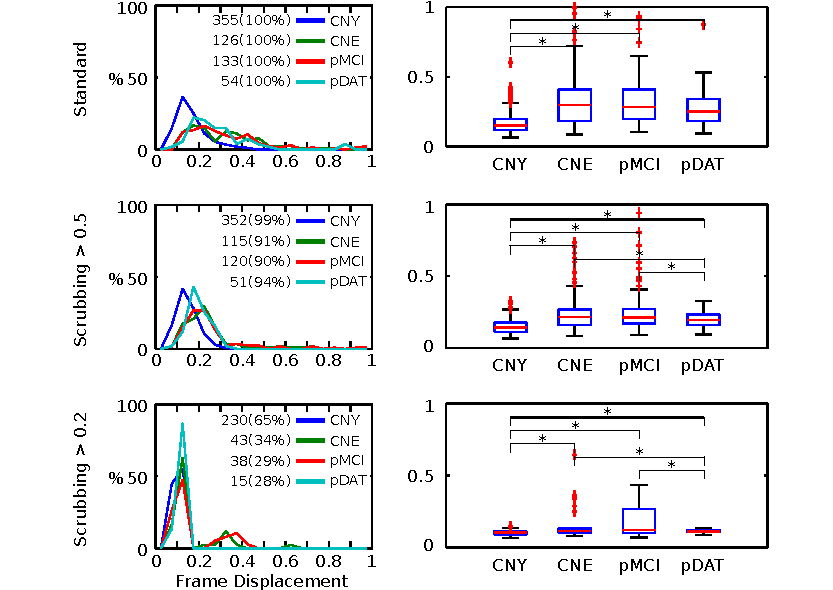
\includegraphics[width=\linewidth]{../figures/figure_fd_distrib.pdf}
\end{center}
\caption{
Distribution of the frame displacement (FD) for 3 groups (CNE, pMCI, pDAT) when scrubbing is applied at various levels (no scrubbing, scrubbing of $FD>0.5$ and scrubbing of $FD>0.2$). The figures on the right depict a boxplot representation of the distributions with there associated statistical differences $t$-test (marked with a {\bf *} for a $p<0.05$).
}
\label{fig_dist}
\end{figure}



\section{Table Legend}

\clearpage
\appendix


%% SUPPLEMENTARY MATERIAL
\clearpage
\pagebreak
\renewcommand{\thefigure}{S\arabic{figure}}
\renewcommand{\thetable}{S\arabic{table}}
\setcounter{figure}{0}
\begin{center}
\emph{Supplementary Material {--} Feasibility of multi-centric fMRI connectivity studies of Alzheimer's disease}\\

\vspace{\baselineskip}Submitted to Neuroimage.\\

\vspace{\baselineskip}C. Dansereau$^{1,2}$,  C. Risterucci$^{3}$, E. Merlo Pich$^{3}$, D. Arnold$^{4}$, P. Bellec$^{1,2}$\\

\end{center}
$^1$Functional Neuroimaging Unit, Centre de Recherche de l'Institut Universitaire de G\'eriatrie de Montr\'eal\\
$^2$Department of Computer Science and Operations Research, University of Montreal, Montreal, Quebec, Canada\\
$^3$F. Hoffmann-La Roche Ldt., Basel, Switzerland\\
$^4$NeuroRx, Montreal, Quebec, Canada\\

For all questions regarding the paper, please address correspondence to Pierre Bellec, CRIUGM, 4545 Queen Mary, Montreal, QC, H3W 1W5, Canada. Email: pierre.bellec (at) criugm.qc.ca.\\

\section*{Literature review: Alzheimer’s disease and resting-state fMRI} 
\begin{itemize}
\item \cite{Zhang2009a} used functional connectivity maps with a seed in the posterior cingulate cortex (PCC) to explore the differences between a group of elderly cognitively normal subjects (CNE, n=16) and patients with a mild dementia of the Alzheimer’s type (DAT, n=18).

\item \cite{Zhang2010} generalized the \cite{Zhang2009a} study with CNE (n=16) and a larger group of patients with DAT (n=46). Patients were separated in three groups (mild, moderate, severe DAT), and each group of patients was contrasted against the CNE.
\item \cite{Wang2006a} used functional connectivity maps with a seed in the hippocampi to explore the differences between a group of CNE (n=13) and patients with a mild DAT (n=13). All results included in the meta-analysis are from Table 2, seeded in the right hippocampus. Seeds were manually delineated on an individual basis.
\item \cite{Wang2007a} used functional connectivity maps with a seed in the posterior cingulate cortex (PCC) as well as full brain point-to-point correlations (based on an AAL parcellation) to explore the differences between a group of elderly cognitively normal subjects (CNE, n=14) and patients with a very mild to mild dementia of the Alzheimer’s type (DAT, n=14). Only the results based on the PCC seed were included in the meta-analysis.
\item \cite{Goveas2011} used functional connectivity maps with a seed in the hippocampi to explore the differences between a group of elderly cognitively normal subjects (CNE, n=18) and patients with a mild dementia of the Alzheimer’s type (DAT, n=14) before and after donepezil treatment. Seeds were manually delineated on an individual basis, before and after treatment.
\item \cite{Damoiseaux2012} used dual-regression independent component analysis to explore longitudinal differences between a group of CNE (n=18) and patients with DAT (n=21). All results included in the meta-analysis are from Table 3 (differences at baseline) and Table 4 (interaction with time). The authors used three components representing the Anterior DMN, Ventral DMN and Posterior DMN.
\end{itemize}


\pagebreak

\begin{figure}[!ht]
\begin{center}
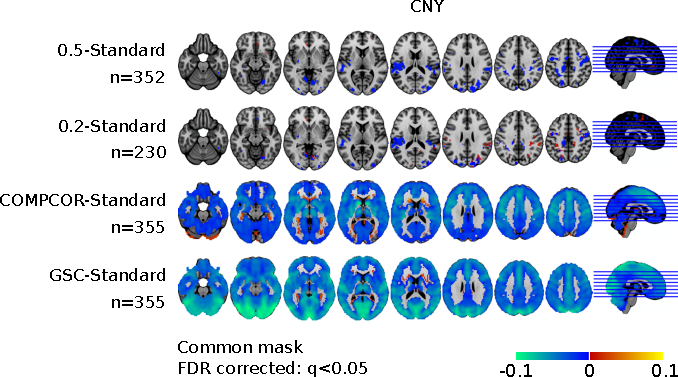
\includegraphics[width=\linewidth]{../figures/figure_comp_cny.pdf}
\end{center}
\caption{
{\bf Differences in functional connectivity for the default mode network (seed in the PCC). Differences in connectivity between all the CNY with scrubbing ($FD>0.5$ and $FD>0.2$), CompCor, and GSC. The mask used depict only significant result of the $t$-test (FDR correction $q<0.05$) only the two scrubbing procedures use the union of there respective mask (common mask).}
}
\label{fig_sup_scrubbimpact_cny}
\end{figure}

\begin{figure}[!ht]
\begin{center}
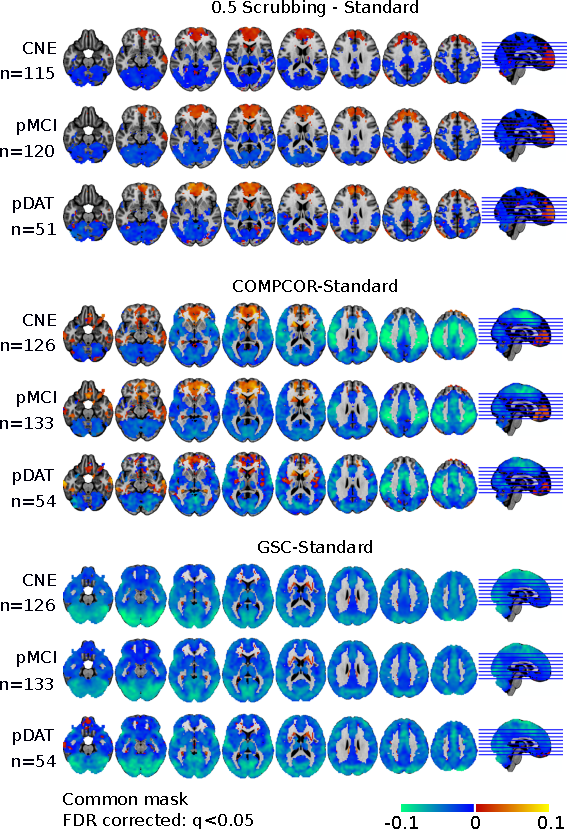
\includegraphics[width=0.75\linewidth]{../figures/scrubbing_impact_cne_mci_dat_all.pdf}
\end{center}
\caption{
{\bf Differences in functional connectivity for the default mode network (seed in the PCC). Differences in connectivity for each group (CNE, pMCI, pDAT) compared to basedline (standard preprocessing) with and without scrubbing ($FD>0.5$ and $FD>0.2$) (FDR correction $q<0.05$) for all voxels showing a significant effect in at least one of the contrast.}
}
\label{fig_sup_impact_on_groups}
\end{figure}



% \begin{table}[!ht]
% \begin{center}
% \includegraphics[width=\linewidth]{../figures/tab_fdr.pdf}
% \end{center}
% \caption{
% {\bf Summary of the empirical false-discovery rate of GLM-connectome (with group or BH FDR), NBS and MDMR on simulations.} {Etc.} 
% }
% \label{tab_fdr}
% \end{table}


\end{document}


